%\documentclass[AER, draftmode]{AEA}
 \documentclass[oneside,12pt]{article}

% \usepackage{soul}
% \usepackage{natbib}
% \usepackage{hyperref}
% \usepackage{graphicx}             
% \graphicspath{{./paper/Figuras/}}

% \usepackage{float}                
% \usepackage{amsmath}
% \usepackage{amscd}
% \usepackage{amsfonts}
% \usepackage{amssymb}
% \usepackage{bbm}
% \usepackage{booktabs}
% \usepackage{nameref}
% \usepackage{multirow}
% \usepackage[nokeyprefix]{refstyle}
% \usepackage{rotating}
% \usepackage{threeparttable}
% \usepackage{lscape}
% \usepackage{enumerate}
% \usepackage{afterpage}
% \usepackage{caption}
% \usepackage{subcaption}
% \usepackage{epstopdf}
% \epstopdfDeclareGraphicsRule{.tiff}{png}{.png}{convert #1 \OutputFile}
% \AppendGraphicsExtensions{.tiff}

% \epstopdfDeclareGraphicsRule{.tif}{png}{.png}{convert #1 \OutputFile}
% \AppendGraphicsExtensions{.tif}

% \usepackage{tikz}
% \usetikzlibrary{shapes.geometric, arrows}
% \usetikzlibrary{calc}

% \usepackage{colortbl}

% \newtheorem{theorem}{Theorem}
% \newtheorem{claim}[theorem]{Claim}

\onehalfspacing

%%% HELPER CODE FOR DEALING WITH EXTERNAL REFERENCES
\usepackage{xr}
\makeatletter
\newcommand*{\addFileDependency}[1]{
  \typeout{(#1)}
  \@addtofilelist{#1}
  \IfFileExists{#1}{}{\typeout{No file #1.}}
}
\makeatother


\newcommand*{\myexternaldocument}[1]{
    \externaldocument{#1}
    \addFileDependency{#1.tex}
    \addFileDependency{#1.aux}
}

%\myexternaldocument{OA}
%----------------------------------------------------------------

\begin{document}

\begin{titlepage}
\title{Information and Lawyer Quality: Evidence from a Field Experiment in a Mexican Labor Court\thanks{We thank Isaac Meza, Sergio Lopez, Enrique Miranda and Ricardo Olivares for research assistance much more valuable than any monetary compensation they received. We also thank the Economic Development and Institutions program, funded by the UK Department for International Development, the GLI program funded by JPAL/ MIT, and the Asociación Mexicana de Cultura for generous funding. Finally, this research would not have been possible without the incredible cooperation of the Mexico City Labor Court, in particular the President of the Court, Darlene Rojas.}}
\author{Joyce Sadka\thanks{Instituto Tecnológico Autónomo de México} \and Enrique Seira\thanks{Instituto Tecnológico Autónomo de México} \and Christopher Woodruff\thanks{University of Oxford}}
\date{\today}
\maketitle
\begin{abstract}
\noindent Does informing plaintiffs about expected case outcomes lead them to hire better quality lawyers? We conduct a randomized field experiment with the Mexico City Labor Court to provide statistical predictions and meetings with court conciliators to potential plaintiffs. Almost all potential plaintiffs are first-time users of the court, who commonly contact a lawyer through private intermediaries looking for clients at the entrance to the court building. On random days, we provide one of three treatments to dismissed workers approaching the court. In one arm, we provide very basic information about the process of filing a lawsuit at the court; in a second arm, we add personalized predictions of case outcomes based on machine learning models drawing from historical case files; in the third arm we add a letter of appointment with a court conciliator, to be delivered by the worker to the firm. We find that providing information on case outcomes does not change the likelihood of filing a suit but increases the quality of the lawyer hired. Adding the letter of appointment with the conciliator reduces the likelihood the worker files a suit and increases the quality of the lawyer hire conditional on filing a suit. We measure the quality of lawyers through both subjective and objective measures. Using these measures, we show that lawyers contracted through intermediaries at the entrance of the court are low quality lawyers. We find that the effect of providing information works mainly through a reduction in the percentage of subjects who hire a lawyer through these intermediaries.\\
\vspace{0in}\\
\noindent\textbf{Keywords:} key1, key2, key3\\
\vspace{0in}\\
\noindent\textbf{JEL Codes:} key1, key2, key3\\

\bigskip
\end{abstract}
\setcounter{page}{0}
\thispagestyle{empty}
\end{titlepage}
\pagebreak \newpage




\doublespacing


\section{Introduction} \label{sec:introduction}
Effective legal representation is crucial for parties to legal cases. Research shows that the quality of lawyers representing plaintiffs and defendants has a substantial effect on case outcomes (Abrams and Yoon, 2007; Anderson and Heaton, 2012). The most credible existing evidence comes from situations where lawyers are assigned randomly to defendants or plaintiffs. However, most parties to cases contract lawyers themselves rather than being randomly assigned a lawyer. Much of the time, at least one party to a legal proceeding is a first-time user of the courts, and hence may be naïve to the legal processes and likely outcomes. This naivety may lead to mistakes in the choice of a legal representative. In this paper, we approach the lawyer-client matching problem by asking whether increasing the information available to clients before they contract with a lawyer results in the clients hiring higher-quality lawyers. 

In Mexico as in many other countries, labor disputes are one of the most common points of contact between individuals and the legal system. Labor laws often provide workers with some compensation in the event of unfair dismissal. Employers and dismissed employees often disagree on whether the worker is entitled to compensation. In the US, these disputes revolve around eligibility of unemployment compensation. In Mexico, dismissed workers are compensated through lump-sum severance payments plus lost wages, and disputes are presently handled in specialized administrative labor courts\footnote{A reform of the labor law passed in 2019 will close down all these executive branch labor courts by 2023 and move labor justice into the judicial branch at both federal and state levels.}. 

All workers filing suits in Mexico’s labor courts must be represented by a lawyer. Dismissed workers may find a lawyer directly, for example, through family and friends, or they may go to either the public attorney’s office or the labor court seeking information and advice. At the Mexico City Labor Court (MCLC), where we conduct our experiment, workers approaching the court are met on the courthouse steps by a group of intermediaries who compete to sign them up with lawyers paying them “finders fees.” This is the first and, often, the only source of information these workers receive about the legal process before committing to a lawyer and filing a suit. Popular wisdom is that these intermediaries often attempt to convince workers to sue even if they have a weak case, because the fees lawyers charge to file a case represent a lucrative return on the time required to do so. Our data will show that use of these intermediaries results in both lower-quality cases and other types of more nefarious abuse. 

Working with the leadership of the MCLC, we established an information booth on the steps of the court. At the booth, we provided basic information about the rights of dismissed workers and the process of legal filings at the court. We also conducted a short survey with the dismissed workers to collect information about their previous employment - wage rate, tenure, and the like - and expectations about outcomes conditional on filing a lawsuit. On randomly selected days, we also provided one of two other treatments. The first treatment provided worker-specific predicted case outcomes based on machine learning models of 5,000 historical case filings and the characteristics of the worker gathered in the short survey. The second treatment provided the same customized predicted case outcome and, in addition, a letter of appointment with a court-employed conciliator addressed to the worker’s former employer\footnote{The two treatments are part of a broader set of experiments we conducted with the MCLC. Two additional experiments are described in Sadka et al (2019). The additional treatments are described in the appendix and left for future work.}. 

We are interested in whether dismissed workers make better decisions when they are more informed. We ask whether these treatments affect the probability that the worker settles with the employer before suing, and whether the workers hire a higher-quality lawyer conditional on filing a suit. In a previous paper (Sadka et al 2019), we report on case outcomes from experiments providing predicted outcomes, intervening at various stages of the process, including in ongoing cases. The data from the experiments with ongoing cases indicate that lawyers do not always represent the interests of their clients. The evidence of agency issues in ongoing cases motivated our design in the experiment reported here, where we work with potential plaintiffs who had not yet hired a lawyer. We expect to find effects on two margins. First, if plaintiffs sometimes file cases that are sufficiently weak that they should not have been filed, making the worker better-informed might reduce the likelihood a case is filed. Second, workers may hire higher-quality lawyers when they do file a case. Of course, effects on the first margin cause selection issues in interpreting effects on the second, and we discuss how we address those below.  

Our analysis uses a combination of survey and administrative court records. We show first that the dismissed workers arrive at the court with expectations that are unrealistically optimistic. For example, 44 percent of workers in the baseline survey say they are 100 percent certain they will win the lawsuit conditional on filing. The statistical information received by the two treatment groups tempers these expectations somewhat. Data from follow-up surveys conducted by telephone two weeks and two months after the initial interaction show that the most intensive treatment increases the probability the worker settles with her employer before filing a suit. Matching workers to administrative records allows us to show that the treatments also affect the quality of the lawyers hired by workers who do ultimately file a suit. 

We face the significant challenge of measuring the quality of the lawyers. One option is to wait until the cases are all completed and measure the effects on outcomes. There are at least two concerns with measuring quality in this manner. First, higher quality lawyers may handle more difficult cases (Dranove et al, 2003). Second, cases proceeding to judgment may take four years or longer to be completed (Sadka et al., 2019); hence we would need to wait a very long time to measure outcomes. Instead, we measure the quality of the initial case filings\footnote{Measuring the quality in initial case files is a good first approach to measure both case file and lawyer quality because it is a crucial document that determines the principal action in the case, as well as the alleged facts. It is also fairly short, and available at the very beginning of the lawsuit, which allows us to rate both historical casefiles and ongoing casefiles with the same methodology.} , which we view as being determined by the quality of the lawyer and the ability of the plaintiff to monitor the lawyer. Our measure of the quality of the initial case filing is grounded in an incentivized, blind rating of case files by eight lawyers with experience litigating in labor court. We describe this exercise in more detail in Section III below. 

There is a literature from U.S. cases that examines the effect of mediation and legal representation on civil and criminal case outcomes. Much of this literature is descriptive, with associations that are not well identified. Greiner and Matthews (2016) review the small number of randomized evaluations in the U.S. courts, finding 50 studies conducted between 1963 and 2015. Mediation and alternative dispute resolution are the most common programs evaluated. The results of the studies are mixed. Mandell and Marshall (2002) find positive effects of mediation in worker compensation cases in Baltimore. However, Clark et al (1995) and Kobbervig (1991) find no effects in civil cases in North Carolina and Minnesota, respectively. Greiner and Matthews report even fewer randomized evaluations on programs that affect the use of lawyers. Greiner and Pattanayak (2012) find no effect of using lawyers on win rates of plaintiffs in unemployment insurance appeals in Massachusetts, but Seron et al (2001) find that lower-income tenants benefit significantly from being represented by lawyers in housing cases New York City. 

None of the fully experimental studies examines heterogeneity of effects by lawyer quality. However, there are quasi-random or non-random studies that examine the effects of lawyer quality on outcomes. Anderson and Heaton (2012) use random assignment of public defenders in Philadelphia to defendants accused of murder to show that, compared with court-appointed private lawyers, public defenders have higher acquittal rates and obtain shorter sentences for their clients. Abrams and Yoon (2007) use random assignment of lawyers to criminal cases within the public defender’s office in Las Vegas to show that public defenders with more experience obtain better outcomes for those they defend. Miller et al. (2015) use data from 20 years of immigration asylum cases to study the relationship between lawyer characteristics and case outcomes. While there are potential issues with the matching of cases to lawyers\footnote{They attempt to correct for potential endogeneity in the way cases are assigned to lawyers using a Heckman selection regression, but is it not obvious that any of the first stage regressors meet the exclusion restriction.},  their results indicate that lawyers who have won a higher percentage of their cases in the past obtain a higher percentage of favorable outcomes. They also show low-quality lawyers do more harm than good: asylum applicants are better off representing themselves rather than being represented by a low-quality lawyer.

While to the best of our knowledge, this is the first experiment that provides information to clients prior to their matching with an attorney, there is a large literature on the effect of information on individual decisions in other contexts. Anagol et al. (2017) conduct an audit experiment in the Indian life insurance market showing that agents use their informational advantage to induce clients to make decisions that are favorable to the agent’s interest. Andrabi, et al. (2017) and Belot, et al. (2018) examine the role of information in private markets, and Jensen (2010) and Dizon-Ross (2019) show that information affects schooling decisions. Information has also been shown to be useful in improving political institutions (Chong et al. (2015); Reinikka and Svensson (2011)). 

We begin by describing the context in which we are working, including a description of the court and the cases that the workers file. Section 3 then describes the experimental design and Section 4 our measures of lawyer quality. Section 5 presents the main results, and Section 6 concludes. 

%-----------------------------------------------------------------

\section{Context} \label{sec:context}
\emph{The law, the court, and the workers}\\
Mexico has a single federal labor law. Federal labor courts apply the law to workers and firms in a group of “strategic industries’’ – oil, gas, and banking, for example. Cases involving other sectors are handled by state-level labor courts that operate in each of Mexico’s 32 states. We work with the state-level court serving Mexico City. The Mexico City court is one of the largest courts in Latin America, with over 100,000 active cases and more than 30,000 new cases filed each year. More than 95 percent of the cases the court handles are “unfair dismissal’’ cases, with employees claiming they did not receive the severance payments owed to them according to Mexican labor law. Firms are not required to make severance payments for "justified dismissals,” but the law provides few valid legal bases for dismissals. For example, low productivity or poor market conditions are considered unfair dismissal and require employers to make severance payments. By law, the severance payment is a minimum of three months' wages, including benefits\footnote{Certain categories of workers are eligible for additional payments. For example, “at-will workers” – those in positions requiring a high level of trust – are also entitled to 20 days wages for each year they worked at the firm.}. 

On paper, the labor law is very protective of workers. However, administrative inefficiencies and delays, a low information environment, and moral hazard from private lawyers, makes workers very vulnerable. In cases where workers win a legal judgment, they collect nothing 53 percent of the time. In the remaining cases where they win and recover a positive payment, they collect on average only 37.5 percent of their claim. Firms have many methods to avoid payment, for example, by closing the business or transferring assets to another entity. This means that in expected value terms, the worker recovers only 18 percent of her claim even when she wins the case. Moreover, trials going to judgment have very long durations, both because the court is overloaded and because defendants are able to delay proceedings: 30 percent of the cases filed in 2011 had not finished by December 2015; among those that had concluded in a judgment, the average duration was 2.5 years. The average duration was almost a year even where cases were settled.

Many of the workers suing are not aware of these problems. Data from a survey we conducted in 2016 (see Sadka et al 2019) with a sample of plaintiffs in ongoing MCLC cases show that only one-third of plaintiffs understand that they are entitled to a minimum of 90 days of salary. The allowance or 90 days severance pay is a right so basic that it is mandated in the Mexican constitution and the concept is taught in standard primary school curriculum. As we will show later in the paper, plaintiffs arriving at the court are wildly optimistic, relative to reality, about their chances of winning their case. Moreover, they have little idea how much they might win\footnote{In Sadka et al. (2019), we found that the subjective probability of winning for plaintiffs and defendants in the same case sums to 1.47. Surveys conducted for that project show that ignorance of plaintiffs extends even to their own lawsuit: only half know what they are claiming in terms of severance, vacation, extra hours, etc. Workers represented by private lawyers are particularly likely to be misinformed.}.

\emph{The lawyers and how workers find them}\\
Workers may be represented in the MCLC by either private or public lawyers. About 20 percent of cases are handled by public lawyers. By law, public lawyers provide legal advice and representation to any worker who requests their help and who has not already hired a private attorney. Public lawyers are formally employees of the city’s Secretary of Labor, and their services are free to plaintiffs. They are paid a flat wage by the city government. Each public lawyer handles about 400 case files concurrently. Private lawyers manage 80 percent of cases field in the court. Although they must be licensed, obtaining the license is fairly easy and private lawyers are generally unregulated\footnote{There is no bar exam, and malpractice litigation is costly and uncertain, with very few known cases of a lawyer losing her license to practice due to a successful suit.}.  Thousands of private lawyers handle cases in a given year at the court, each managing around 50 cases simultaneously. Private lawyers typically charge plaintiffs an initial fee of about MXN \$2000 pesos (USD 100) to file the lawsuit and a contingency fee of about 30 percent of any amount collected by the plaintiff. In spite of the contingency fee, their incentives are not perfectly aligned with those of their clients. First, while plaintiffs are party to a single case, the lawyers manage a portfolio of many firing lawsuits with widely differing characteristics, against many different firms. With diversified risk, they may be more willing to take risks on any given case. Second, filing a low-quality suit is cheap and easy and the lawyers may profit from collecting the filing fee even with no expectation of recovering anything on behalf of the worker. 

Lawyer’s education and quality varies widely\footnote{Former minister of Mexico’s supreme court Cossio Diaz has “Questioned the existence of more than 2000 law schools at the national level, that there is no encompassing lawyer association, and the low quality standard of the profession.’’ (https://www.jornada.com.mx/2014/02/12/politica/020n1pol).}.  The strategies they follow and the case outcomes also vary. Controlling for case observables, lawyer fixed effects explain 44 percent of the variance of recovering a positive amount on a case, 45 percent of the variance in settlements, 49 percent of case duration, and 65 percent of whether or not they add a social security claim to the firing claim. Figure 1 shows the variance of outcomes across lawyer offices in two measures of the amount recovered in cases. However, under the current institutional structure it is hard for workers to ascertain the quality of lawyers. As we noted, almost all plaintiffs are first-time users of the court\footnote{In surveys carried out in a related project (Sadka et al. 2019), we find that plaintiffs have little experience in labor suits, with 82 percent of cases having workers suing for the first time.}.  There is no database workers can consult for lawyers and their outcomes, so plaintiff’s lawyers have weak incentives to acquire reputation. And finally, ignorance and overconfidence may make workers easy prey to lawyers. As we will show below, lawyers contracted through intermediaries outside the court building – a common practice for plaintiffs approaching the court – appear to be of particularly low quality.

Choosing the right lawyer is critical because, once a case is filed, lawyers control the lawsuits almost completely. All lawyers require the workers they represent to sign a power of attorney. The standard power of attorney gives broad powers to the lawyer, including dropping the lawsuit with the worker being present to ratify the decision\footnote{In August 2017 the Mexican Supreme Court created jurisprudence stating that in labor lawsuits, when a worker has signed a broad power of attorney allowing her lawyer to drop the lawsuit on her behalf, then the lawyer can drop the suit without the presence or ratification by the worker, see \url{http://sjf.scjn.gob.mx/SJFSist/Paginas/Reportes/ReporteDE.aspx?idius=27262&Tipo=2&Tema=0}, accessed 30 August 2019.}.  Also, the court procedures do not oblige the worker herself to attend any hearings, except to provide her own deposition, should that be required as evidence. The importance of the choice of lawyers is also indicated by evidence that some lawyers may not take the actions that best represent their clients’ interests. Sadka et al. (2019) provide evidence of agency issues in representation, and show that in 40 percent of lawsuits, workers pay more than they receive, in the sense that what they recover is lower than the fees they pay the lawyers (and this even without taking into account the effort, stress and risk workers incur). We also show evidence below that lawyers sometimes file suits without plaintiffs knowing. 

\begin{figure}[!htbp] %Falta arreglar caption--------------
    \caption{Lawyer fixed effects, controlling for variables of the case}
     \begin{center}
    \begin{subfigure}{0.49\textwidth}
        \caption{Amount won as a percentage of amount asked}
        \centering
        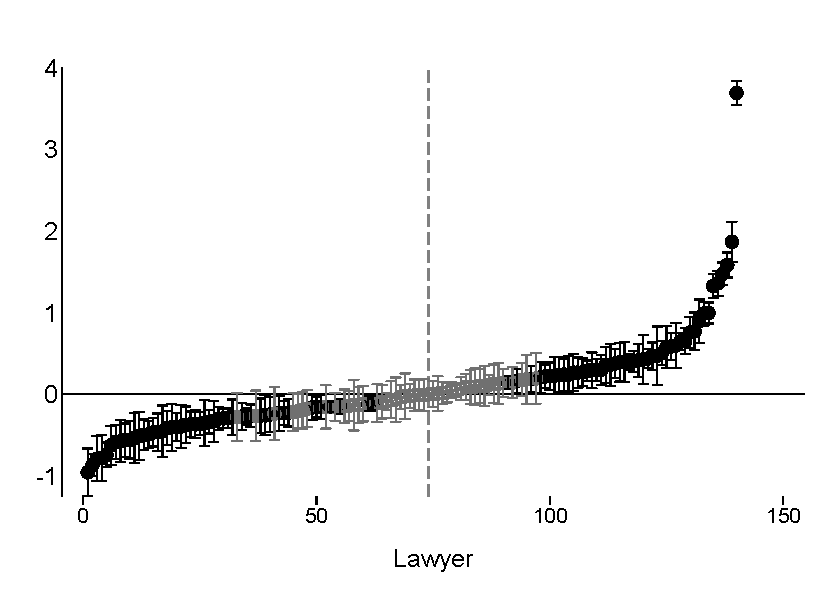
\includegraphics[width=\textwidth]{Figuras/betas_ql_win_minley.pdf}
    \end{subfigure}
    \begin{subfigure}{0.49\textwidth}
        \caption{Recovered a positive amount}
        \centering
        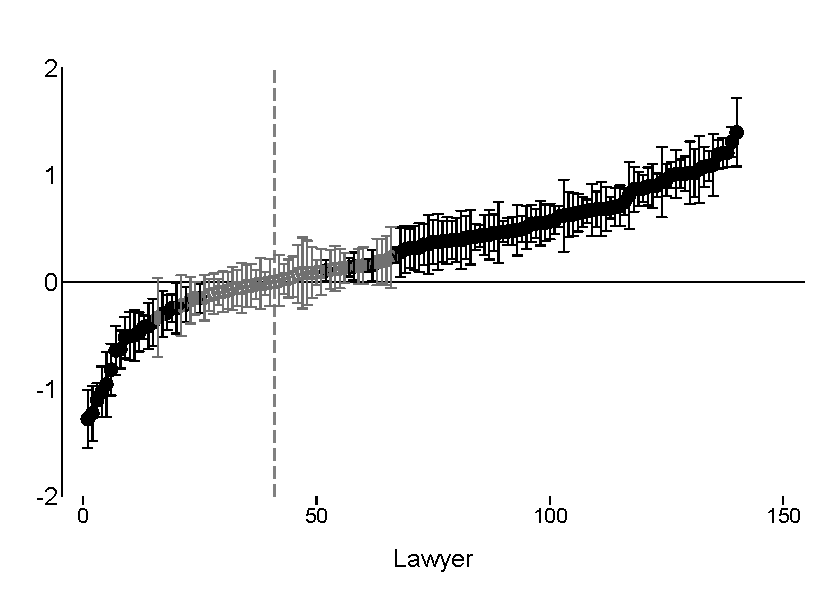
\includegraphics[width=\textwidth]{Figuras/betas_ql_pos_rec.pdf}
    \end{subfigure}
    \end{center}
    \scriptsize{ \noindent Panel (a): Dependent variable is the amount won divided by the law minimum. Each coefficient corresponds to a different law firm dummy. Panel (b): Dependent variable is an indicator of winning a positive amount. Each coefficient corresponds to a different law firm dummy. The regression controls for variables of the case.
    \textit{Do file: }  \texttt{fe\_quality\_betas.do}}
    \label{fig:1}
\end{figure}
%----------------------------------------------------------

How do plaintiffs find their lawyer? Workers typically follow one of three paths. Some dismissed workers will contact a private law firm directly. They may either have sued previously or know someone who recommends a particular lawyer. Others will go to the public attorney’s office directly. Finally, a third group will come to the labor court building seeking information. The court itself does not typically provide any legal advice. Instead, at the court, the dismissed workers will encounter the intermediaries who we have described, and who may pass on to a lawyer them to a lawyer. Our sample, and the group for whom we have direct information from surveys, comes from the third group. This is obviously not a representative sample of either dismissed workers, or of workers filing suits. We will use data from the Mexican quarterly labor survey to compare our sample to the broader sample of dismissed workers\footnote{We also intend to compare our sample to all workers filing cases in a future version of the paper.}.

\section{Experimental Design, Treatments, and Data} \label{sec:data}
The experiment was conducted with full cooperation of the Mexico City Labor court and was run between May 2017 and August 2018. The population of interest is dismissed workers approaching the MCLC in search of information about their rights and how to file a lawsuit. We describe the sample in more detail below. Working with the court, we established an information booth at the entrance of the court. To increase visibility, the booth was announced on a large banner on the wall of the court building. Given the high level of visibility of the information booth, we believe that essentially all dismissed workers coming to the court were aware of the availability of free information. However, approaching the booth for information was optional. We estimate that around one third of those coming to the court stopped at the booth. 
\[\]
\noindent\emph{Description of treatments}\\
Workers approaching the information booth at the court were met by research assistants with a degree in law. The research assistants carried out one of three protocols, with each randomly assigned to one of the protocols on a weekly basis. All workers approaching the booth on a given day were treated in the same way. 

\emph{Control condition}: The first protocol is the control group. We first administer a short survey. Then we provide workers with a schematic map of the court and basic information about the items that are included in the calculation of severance payments in case of dismissal for causes other than delinquency. We provide a copy of the brochure in Appendix B Figure \emph{i}\footnote{When we started the project in May 2017, the control condition was simply to administer the survey. But we found that many individuals were unwilling to answer the survey. The survey rates increased markedly when we added the basic information. The trade-off is that the basic information may be a light treatment itself.}. 

\emph{Personalized information}: On days assigned to the personalized information treatment group, we provided a more detailed version of the information on legal rights and processes than we provide for the control group. Appendix B Figure ii provides a copy of the information on legal rights and procedures that we give to workers. The explanation included providing them with the correct definitions of justified and unjustified dismissal under Mexican labor law, details of how to calculate the total severance pay owed to them, and information about what options they had for finding a lawyer and filing suit. This information is needed for them to be able to interpret the ``calculator’’ information we also provided.

We then asked workers for additional information about their employment contract, hours, and fringe benefits. We use these, along with the baseline survey, to make a personalized prediction of their case outcome. The predictions are derived from applying machine learning predictive models to 5,000 historical cases. We provide workers with a printout (see Figure 2 below) that contains four relevant pieces of information. First we repeat the relevant details of their personalized employment relationship, so that they can verify that the prediction is based on the correct information. Next we present the 25th and 75th percentiles of the settlement amounts in the historical cases matched to their characteristics, telling them that “the majority of settlements are in the range…” between these two numbers. We report these as the number of days of their salary. The third and fourth pieces of information are the percentage of cases proceeding to court judgment that are not resolved three years after filing and the percentage of cases proceeding to judgment in which the worker receives no payment. The machine learning models used in the personal prediction calculator are detailed in the appendix to Sadka et al. (2019). 

It is important to note that in the text of the personalized calculator, received by both calculator and calculator+letter treatment groups, we include a phrase stating that the uncertainty involved in carrying out an entire labor lawsuit makes conciliation talks in search of a settlement an attractive strategy for both parties. As will be seen in our results, notwithstanding this clear message, the effects on conciliation are much stronger for workers in the calculator+letter group, perhaps indicating that without providing workers with a clear immediate course of action, the effects of the calculator on settlement behavior is far smaller.

\begin{figure}[!htbp] %Falta arreglar caption--------------
   \begin{center}
   \centering
    \caption{Personalized calculator printout}
    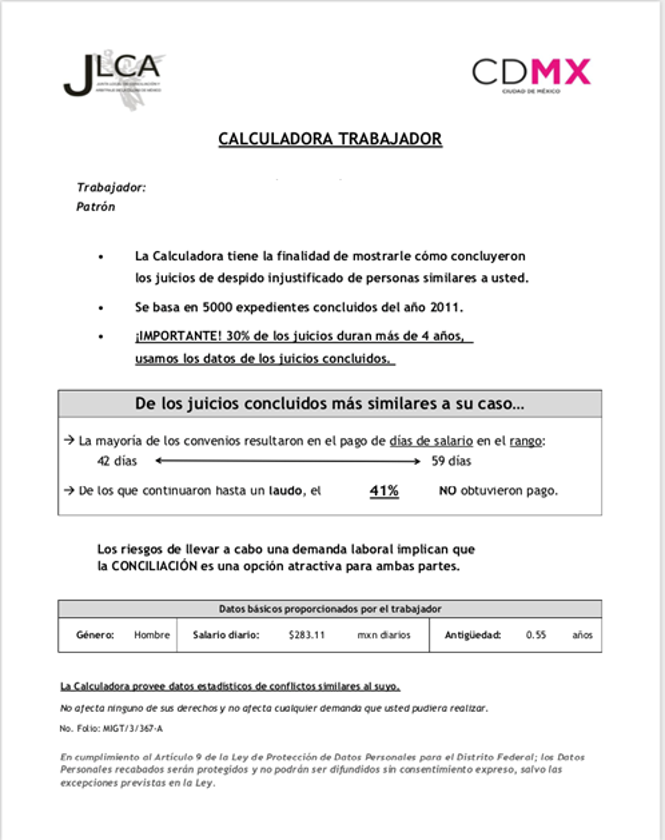
\includegraphics[width=0.8\textwidth]{Figures/Figure2.png}
    \label{fig:2}
    \end{center}
\end{figure}
%----------------------------------------------------------

\emph{Personalized information and a letter of appointment}: On days allocated to the third protocol, we provided workers with the same treatment as in the personalized information arm, and in addition. we provided them with a letter addressed to their ex-employer. The letter gave both the worker and the employer an appointment with a court conciliator at the MCLC for a date around one week after treatment. Appendix 2 Figure iii contains an example of the letter, and an English translation of the same. The letter specifies the date and time of the appointment. The employer is also informed that the ex-employee has received statistical information on expected case outcomes, and that the employer will receive this information after arriving at the appointment. The worker was then asked to give the letter to their employer, and we called both the worker and the firm to verify whether the letter was delivered and to confirm their attendance at the appointment. When both parties appeared for the appointment, we provided calculator information to the firm’s representative and then left them in a conciliation office with one of the court conciliators, to conduct settlement negotiations in private. 

\emph{The sample}: During the course of the experiment, just under 3,000 dismissed workers approached the information booth and completed baseline surveys. Table 1 shows the summary statistics from the baseline survey by treatment arm. The sample is well balanced across treatment arms. About 68 percent of each group have finished high school, 45 percent are female. The average wage was 300 pesos per day (close to 15 US dollars), and the average tenure at the firm was three and a half years. The workers are wildly optimistic about their prospects at the court. On average, the dismissed workers believed they had an 89 percent chance of winning their case if it went all the way to a court judgment. By comparison, on average in the sample, the calculator predicts a 24 percent probability of recovering a positive amount conditional on continuing the lawsuit until the court judgment. Conditional on winning they expected to recover close to 190 days of salary. The expectation on the amount they would recover is less exaggerated. Rather, the main story here is one of uncertainty: 42 percent of respondents said that they could not say what that they expected to recover. 

We conduct the experiment on those workers approaching the information booth at the court. As we noted above, dismissed workers might find a private lawyer away from the court, or go directly to the public attorney’s office. Moreover, we estimate that only around one-third of the workers coming to the court stopped at the information booth. As it happened, for most of the period of the experiment, the public attorney’s office was located inside the court building, and hence, workers coming to the public attorney’s office might have stopped at the information booth. An earthquake in September 2017 caused severe damage to the main office building that housed the public attorneys\footnote{The damage to the public attorney’s office provides additional rationale for digitizing records. The public attorney’s office was one of only a handful of buildings in Mexico City that suffered significant damage. Many believe that the damage was due to the weight of the paper records from past cases held in the office.}.  For a period of around a year, most of the public attorneys worked out of offices in the labor court building. This meant that workers could consult with public lawyers at the court. Nevertheless, resource limitations meant that obtaining advice from public lawyers involved long waits, and many workers would opt to talk to informal lawyers, who we will identify as a low-quality category of lawyers, at the court gate or on the court steps, rather than waiting in line for public lawyers.

We can compare our sample with the population of dismissed workers by referring to data from Mexico’s quarterly labor survey\footnote{The \emph{Encuesta Nacional de Ocupacion y Empleo} (ENOE) samples are based on place of residence. Dismissed workers file in the court with jurisdiction over their employer, and the ENOE does not ask for location of employment. Hence, there is some mismatch, as workers residing in Mexico City may work in Mexico State, and vice-versa. Nevertheless, we see the comparison as at least indicative of differences between the population of dismissed workers and the sample of workers in our experiment. }.  Using sample weights for the labor survey, we find 92,000 workers resident in Mexico City were fired from their job during the period of our experiment. In response to a direct question about severance pay, only around 5 percent of the dismissed workers report that they received severance pay. About 29,575 of those workers filed a suit at the MCLC during the same period. Our sample is around 10 percent of the number that file suits, suggesting that around 30 percent of those filing suits came to the court. Since around 20 percent of cases are filed by public attorneys, this suggests that half or more of the dismissed workers who sue find private lawyers directly. 

Table 1 shows averages for several characteristics of workers that are available from our survey, by treatment assignment. We also show averages from the ENOE for workers fired as close as possible to our sample period using Mexico’s employment survey. The data show balance across treatment groups in all of the basic measures (columns 1-3, p-values in column 5). However, we find differences between several variables for workers in our sample and average for dismissed workers in the ENOE. The differences may at first appear surprising: The workers in our sample are more likely to have completed upper secondary schooling (68 percent vs. 27 percent) and reports a higher daily wage (around 320 pesos vs. 220 pesos). The ENOE workers are also more likely to be male. We expect workers coming to the court in search of legal advice would be those with little information and few connections to help them find a good lawyer. Hence, it may be surprising that they are better educated and higher paid than the average dismissed worker. However, a large fraction of workers in Mexico are hired informally. Informal wage workers are lower paid and lower-skilled. They are also likely to realize that they will not be able to recover any severance pay. Hence, the sample of those seeking severance pay is likely to be positively selected form the full sample of dismissed workers\footnote{We are able to compare the workers approaching the court with the full sample of workers filing cases in the court. We plan to code salary, tenure, and other observable characteristics from case files of a random sample of suits during our experimental period, and from the case files of those in our control group filed suits. We aim to include this comparison in a future draft. }.  

%--------------------------------------------
\begin{table}[!ht]
    \caption{Summary Statistics and Balance}
    \label{tab:SS}
    \center
    \scriptsize{% Table generated by Excel2LaTeX from sheet 'Hoja1'
\begin{tabular}{lccccl}
\toprule
\toprule
\multicolumn{6}{c}{\textbf{Experiment summary statistics}} \\
\midrule
      & \multicolumn{3}{c}{Treatment} &       & Balance C-T1-T2 \\
Variable & C     & T2    & T3    & ENOE  & \multicolumn{1}{c}{p-value} \\
\midrule
Finished highschool & 0.67  & 0.69  & 0.68  & 0.265 & \multicolumn{1}{c}{0.59} \\
      & (0.02) & (0.02) & (0.02) & (0.441) & \multicolumn{1}{c}{0} \\
Woman & 0.45  & 0.46  & 0.45  & 0.326 & \multicolumn{1}{c}{0.89} \\
      & (0.02) & (0.02) & (0.02) & (0.469) & \multicolumn{1}{c}{0} \\
Daily wage & 352.04 & 293.51 & 312.07 & 222.7 & \multicolumn{1}{c}{0.16} \\
      & (26.87) & (8.54) & (15.24) & (123.1) & \multicolumn{1}{c}{0} \\
Tenure & 3.65  & 3.74  & 3.67  &       & \multicolumn{1}{c}{0.93} \\
      & (0.16) & (0.15) & (0.19) &       & \multicolumn{1}{c}{0} \\
Exp. Calculator pred.  & 3844.19 & 3373.56 & 3619.49 &       & \multicolumn{1}{c}{0.23} \\
      & (242.04) & (115.33) & (161.84) &       & \multicolumn{1}{c}{0} \\
Prob. winning & 0.89  & 0.87  & 0.89  &       & \multicolumn{1}{c}{0.21} \\
      & (0.01) & (0.01) & (0.01) &       & \multicolumn{1}{c}{0} \\
Amount in daily wages  & 176.51 & 191.47 & 192.74 &       & \multicolumn{1}{c}{0.56} \\
      & (11.37) & (11.06) & (15.54) &       & \multicolumn{1}{c}{0} \\
      &       &       &       &       &  \\
\midrule
Observations & 995   & 995   & 995   &       & 17419 \\
\bottomrule
\end{tabular}%
}
    
    \begin{figurenotes}
    This table shows summary statistics and balance tests for the experimental sample. It displays means and standard deviations for selected variables, and the p-value of an F-test of equality of means across treatment arms. The variables measure the fraction of subjects that finished high school, the fraction of women, average daily wage (in Mexican pesos), and years of tenure in the firm. We also included measures of the “calculator” prediction for the amount recovered (in pesos), the subjective belief about the probability of winning the lawsuit and the amount they expect to recover conditional on winning. The ENOE column uses data from respondents in Mexico City who report being dismissed from a job in the previous three months, weighted to be representative of all residents.
    \end{figurenotes}
    %\textit{Do file: } \texttt{SS_draft}
  
\end{table}
%--------------------------------------------


\[\]
\emph{Data}\\
We use data from a variety of sources in the analysis. These include data from the court’s administrative data, data from surveys, and data from a team of external labor lawyers we hired to rate lawsuits. We describe the data briefly here. 

\emph{Baseline survey}: Each dismissed worker approaching the information module asking for advice filled out a short baseline survey. After piloting, we realized the survey had to be less than 5 minutes long, so we only asked a few questions. The questions included full name, detailed address and phone numbers, gender, wage, tenure, industry, firm name, date the job started, date of firing, how angry the subject was with the firm, and the probability the worker attached to winning in a court judgment if she sued the employer, as well as the amount she expected to win in a court judgment. 

Since many subjects said they could not predict the probability of winning in court, and even more said they could not predict the amount they would win, we elicited their subjective expectations with a two-part question. We first asked: “What is the percent chance that you will win a payment at the end of a labor trial in a scale from 0 to 100, where 0 is impossible and 100 is completely sure.’’ If they could not answer that, then we asked if this percent change is above 75 percent or below. For the amount we asked: “In case you sued the firm that fired you and you won the trial, what peso amount do you expect to be awarded? Again if they could not say, we asked them if this was above or below half a year of their salary. The benchmarks of 75\% or more and half a year’s salary or more were chosen because they are close to the average subjective probability and amount from prior surveys. 

\emph{Immediate follow up survey}: For all the arms except the control, we re-asked the expectations questions about 1 or 2 minutes after they got the information from the calculator and before doing anything else. This allows us to measure immediate expectations and to have these expectations uncontaminated be the passage of time and events. In piloting, we asked the control group an immediate follow-up as well. However, since this was right after the same questions a few seconds later they were thrown off by our re-asking, and they invariably gave us the same answer as before, often expressing some irritation. Therefore, we stopped asking for immediate expectations shortly after starting the experiment.

\emph{Two week follow up survey}: Approximately two weeks after the contact in our module, we conducted a survey by telephone. The main objective was to measure whether the worker had filed a suit, settled, or dropped the case. In case of settlement, we asked for the amount and date. We also asked if they talked to a lawyer, whether the lawyer was public (which we checked by asking where his office was), and if the lawyer was private where and how did they find him. In particular, we asked if they found him at the stairs/entrance of the court; whether he was recommended by friends or family or is a friend or family member; whether he was found through media advertisements or internet, or in any other way. Finally we also asked their subjective expectations about their likelihood of winning and expected amount of money in the same format as before, and about their level of schooling. We are not currently using these expectations since we cannot elicit them cleanly for those that have settled as it would involve an implausible counterfactual\footnote{We piloted, with little success: “if you had not settled what would you expect on a trial if you had sued…”}. 

\emph{Two month follow up survey}: We conducted a second telephone survey two months after the worker approached the information booth. The main objective of this survey was to measure if the worker settled or filed a suit, and if so, with which type of lawyer. The law establishes that the worker has 60 days from the date of dismissal to initiate a labor lawsuit. If this period lapses the right to sue for unfair dismissal expires. Hence, there should be no additional filings after the two-month survey. At two months, we asked whether they sued, settled, or dropped the case, and in case of settlement, amount and date. We also asked if they had hired a lawyer, whether the lawyer was public, and if the lawyer was private where and how they found him. We also asked, with the same wording as in the earlier surveys, about their subjective expectation about their likelihood of winning, and about the amount they expected to collect after a favorable court judgment. If they sued with a public lawyer, we asked whether, prior to filing the lawsuit, the public lawyers’ office provided them with a letter of appointment asking their former employer to appear at a pre-lawsuit settlement meeting, and whether the firm attended the meeting. Finally we asked some questions about strategy in their lawsuit, such as whether they were asking to be reinstated in their jobs or indemnified for the firing.

A second objective of the two-month survey was to measure the worker’s knowledge of the main law entitlement for severance, how satisfied they were with their lawyer, and how angry they were with their previous employer. We also measured whether they are looking for a job, and if not, how likely they believed it was that they would find one. Finally they answered how much time they had spent at the court, talking to lawyers and inquiring about their case, how much money they had spent, how much time it took them to get from their home to the court, and how many visits they had made to the court since being fired.

A third and final objective was to measure proxies for the worker’s welfare. We asked a question about food security, whether they are able to pay for electricity, rent and food. We also included a life satisfaction question modeled on the similar Gallup question.
\[\]
\noindent\emph{Administrative Data}\\
We use data from administrative records of the MCLC for several purposes. First, we collected data from 5,000 cases filed in five MCLC subcourts in 2011. We use these to generate the models of predicted case outcomes, which in turn are used to predict outcomes for participants in the experiment. For each of the five subcourts that were involved in the experiment described in Sadka et al. (2019), we capture data from the initial case filing for the first 1000 cases that were filed in 2011 and completed by December 2015. We also collect data from the court’s digital system on case outcomes for the historical 5000 files. The initial case filing includes measures of the plaintiff’s daily wage rate, tenure with the firm, and the specific claims the plaintiff is making in the case. We use machine learning models to predict the amount of settlements and the probability of collecting a positive amount conditional on the case going to judgment. The models developed from these 5,000 historical cases are then used to predict outcomes for the experimental subjects based on those subjects’ own characteristics. The calculator is described in more detail in Sadka et al. (2019). We also use a subsample of 500 of these 5,000 cases in the case file quality rating exercise that we describe below. 

Second, the court provided us data in electronic format on all of the unfair dismissal cases filed in all 20 subcourts from May 15, 2017 through 2019. These data allow us to match the sample of workers approaching the court with any cases that they file later, a process we describe in detail below. The records show the case file number, the name of the plaintiff and defendant and the date of the filing. We were also provided access to the complete initial case files for all of the cases filed during this period. These case files come as high-quality images that we are able to digitize with some effort. The filings are typically around five to ten pages in length and describe the circumstances of employment - tenure, salary, overtime, etc., and dismissal. Importantly, these files also contain the name of the plaintiff’s lawyers and the compensation sought by the plaintiff.

\section{Measuring lawyer quality: Subjective and objective measurements}
\label{sec:measuring}
The experimental treatments might affect either the decision of the worker to settle, file a suit, or drop the case. Conditional on filing the treatments might also affect the quality of the lawyer chosen by the worker. Anecdotal information indicates that the lawyers hired through the intermediaries operating outside the court building are lower-quality\footnote{https://www.meganoticias.mx/guadalajara/noticia/acechan-coyotes-a-usuarios-junta-de-conciliacion/58814, and https://www.informador.mx/jalisco/Pese-a-modulos-coyotes-continuan-en-la-Junta-Local-20190528-0026.html, The president of the local labor court of the State of Queretaro was quoted as saying that the coyotes provide bad representation to workers, deceiving them to believe that they will win a lot of money with a lawsuit. (http://www.eluniversalqueretaro.mx/metropoli/14-09-2016/alertan-sobre-coyotes-en-junta-de-conciliacion.)}.  For example, in pursuit of the up-front fees from filing a case, the intermediaries are often believed to file cases that have little prospect of recovering any payment. These filings are likely to be “quick and dirty,” of low quality. We are able to identify lawyers hired through intermediaries with our survey question asking workers where they found their lawyer. We find that, at least among the workers approaching the court, use of lawyers hired through intermediaries is common. In our sample, 19 percent of the control group found their lawyer outside the court, through intermediaries. We aim to provide more direct evidence on the variance in quality of lawyers in general, and on the quality of those hired through the intermediaries in particular. We noted in the introduction several challenges to doing this through case outcomes. There is selection: better lawyers may take on more difficult cases (Dranove et al. 2003). There are long delays, as cases proceeding to judgment may take many years to complete. That implies that we could measure the quality of lawyers new to the court only with very long lags. 

Instead, we pursue an alternative approach, based on rating the quality of the initial case filing itself. Discussions with lawyers indicated that case filing varied in quality, with issues related to specificity of the information and claims being the most important. For example, is the address of and other contact information for the defendant complete and detailed? Defendants must be served notice of the suit and hearings, and incomplete information is the most common obstacle to timely notification. Are the circumstances of the dismissal complete, including the names and positions of the individuals who carried out the dismissal? These facts about the dismissal are often the main focus of the evidentiary phase of the lawsuit; greater specificity and clarity are key to lawsuit quality. 

With these issues in mind, we measure the quality of the case filing in four steps. First, we selected a sample of 500 of the 5000 cases filed in 2011 and hired eight licensed lawyers to rate the quality of the initial filing for those cases. Second, we hired two lawyers as consultants. We asked those two lawyers to examine 100 case files and to suggest hard measures that we could objectively code that might be used to judge the quality of the case filing. Third, we code a subset of those 100 objective measures for all of the 500 case files rated by the eight lawyers. We then map the subjective ratings provided by the eight lawyers to the objective measures. The fourth and final step is to code the objective variables for each of the experimental cases, and to use the coefficients generated in step three to generate predicted ratings for each of the experimental case files. We describe each of these steps in more detail in the remainder of this section. 

\emph{Subjective ratings}: We hired eight licensed lawyers to rate the quality of the initial case file from a sample of 500 historical cases. The eight lawyers all currently litigate labor cases and had, on average, about 5 years of experience in litigation. The 500 cases are a stratified random sample of the 5,000 historical case files described above. We anonymized each case file by blocking out information on the names of the lawyers and plaintiffs, and then asked two lawyers to rate each file independently, so that each of the eight lawyers rated 125 case files. Each lawyer accessed her assigned case files through an online platform we developed. The platform provided detailed instructions for providing the ratings, and the interface to enter the ratings\footnote{The instructions for the lawyers proving the ratings is shown in Appendix 4. An English translation will be provided in a future draft.}.  The lawyers rated each of five main parts of the case filing: the introduction; the list of claims; the facts; the legal arguments; and the closing petitions to the court. They also provided a global rating of the quality of the case filing. They were instructed to rate the case filing itself rather than the quality of the underlying case. The instructions clearly mentioned coherence, completeness, specificity, and well posed claims and arguments as the correct basis for the evaluation, rather than the value of the case or the legal merits of the case\footnote{The exercise is similar in spirit to the exercise carried out by Cole et al. (2014), who hired loan officers to rate the riskiness of loans made by an Indian bank.}. 

In addition to the quality rating, we asked the lawyers to “predict” the outcomes of each case file. Of course, because these are historical cases, the outcome was known to us. That allowed us to incentivize the lawyers’ predictions. We made bonus payments for each of the 125 cases if the lawyer correctly predicted the way the case ended - in settlement, in a court judgment with or without positive recovery, by expiry, or by being dropped. We also asked the lawyers to predict the amount recovered conditional on settlement, the amount recovered conditional on a favorable court judgment, and the likelihood the plaintiff was able to collect payment from the defendant conditional on receiving a judgment in favor of the worker. Again, these predictions were incentivized, with lawyers receiving a bonus if they were within 20 percent of the actual amount recovered by the plaintiff, and within 20 points of probability predictions. The bonuses represented almost half of their payment for the exercise. Figure 3 shows that there is substantial variation in the ratings of the case files. 

\begin{figure}[hp]%-------------------------------------------
 \centering
 \caption{Distribution of Subjective Ratings (500 cases)}
 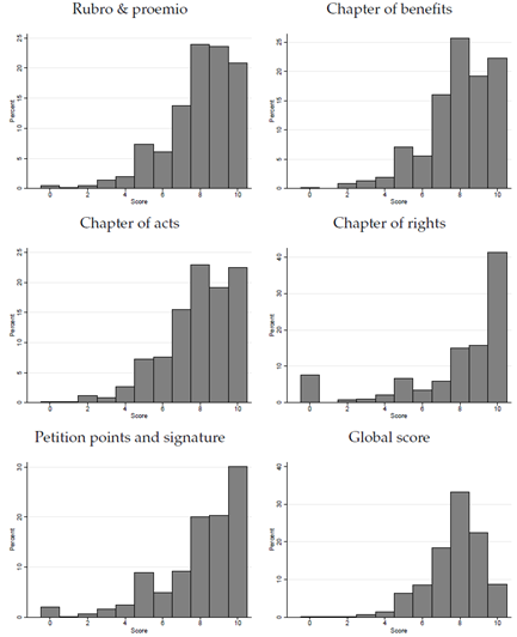
\includegraphics[width=0.8\textwidth]{Figures/Figure3.png}
 \caption*{Notes: This Figure shows distributions of rating for the 500 casefiles by our 8 hired practicing lawyers. We asked for a grade from 0 to 10 in each of the 5 parts of the lawsuits and a global score.}
 \label{fig:3}
\end{figure}%-------------------------------------------------

\emph{Constructing objective measures of quality}: The subjective rating exercise provides a case file quality measure for each of the 500 historical case files. However, we need a way to estimate the quality of the case files for ongoing cases\footnote{We plan to hire lawyers to rate each of the experimental case filings, but as that will take several months to complete, we describe here a method to estimate the quality of these case files using the ratings of the 500 historical case files.}.  With this in mind, the second step was to hire as consultants two lawyers specializing in labor law. We asked the two lawyers to read a random subset of 100 of the 5000 historical case files, and to suggest hard measures that we could objectively code from the case files that might be used to judge the quality of the case filing. They suggested around 100 possible variables, most of which measured the precision of the language used in the case filing. We conducted statistical analysis using regression and principal component analysis, and selected 40 variables, which we coded for each of the 500 case files that had been rated by the eight lawyers. 

These 40 variables include measures of whether the filing correctly specifies the worker’s base salary, salary including benefits, the periodicity of salary, the days worked per week and exact hours worked each day. Clarity in these data contribute to a more precise quantification the worker’s claims in the case. Their inclusion in the filing obviates the need for the court to collect additional information from the plaintiff. This, in turn, speeds up the hearings in the case, and also provides a clearer starting point for settlement negotiations with the defendant. Other variables measure the number of defendants, whether defendants full names and addresses are included in the case filing, the number of plaintiff lawyers listed (proxying the size of the law firm representing the plaintiff), and whether all of the parties’ full names and addresses are given in the filing. Names and addresses of the defendant are particularly important, because mistakes may prevent formally serving (notifying) the defendants, and this can seriously delay the lawsuit. A larger number of defendants is often a precautionary measure by the plaintiff’s lawyer, since the worker may not have a copy of her contract, may have been paid through an outsourcing firm, or may have been an employee of a semi-formal firm, so that suing the firm owner or manager could help raise the chances a worker can later collect on a favorable judgment. 

The variables also include more precise descriptions of the facts surrounding the case. These include whether the worker signed a written contract and whether the worker received a copy of the contract, the exact time, place, and circumstances of the firing, the full name and position at the firm of the person who fired the worker, and the exact reason for the firing, if provided by the firm. Precision in the description of the circumstances of firing may be correlated with the lawyer having discussed the circumstances of the firing in a more detailed way with the worker. Moreover, a more accurate description makes it harder for the defendant firm to refute these facts. When the lawyer does not discuss the facts in detail with the worker, which anecdotally seems to be the case for lawyers hire through intermediaries outside the court, the description of the circumstances of firing will tend to be less detailed and more generic, to avoid refutation by the defendants. The last of the 20 variables contain the final petitions made of the court in the case filing, such as petitioning the court to recognize that the suit was filed within the statute of limitations and that the lawyer has a valid power of attorney allowing her standing to represent the worker in the suit. 

A natural concern is whether the lawyers’ ratings reflect the quality of the case file, or the quality of the underlying case. We note first that the instructions provided to the eight lawyers are clear that we are interested in the quality of the case file rather than the case. Moreover, we are able to provide additional evidence on this question because we know the outcomes of the 500 cases. In addition to rating the case filing, we also asked lawyers to predict the probability the case ends in each of 5 ways (e.g., settlement, win in court, drop, etc.), and the amount won / collected for each outcome. We use these to construct a measure of the lawyer’s predicted (weighted) case outcome. When we regress the actual amount collected on the case file rating alone, we find that the case file rating – the average rating of the two lawyers – positively predicts the amount collected. However, when we add the average weighted outcome predicted by the lawyers, the case file rating loses significance, while the predicted outcome is strongly predictive of the actual case outcome\footnote{Results available from the authors. Interestingly, the coefficient on the lawyer’s predicted collection is very close to 1, suggesting that the lawyers got the prediction right, on average. (See Appendix 4.)}.  We read these results as supporting the supposition that the lawyers engaged in two quite different exercises when they rated the quality of the case file and the strength of the underlying case itself. 

\emph{Predicted ratings for experimental case files}: The third step is to code the 40 objective measures for all the 500 case files rated by the eight lawyers, and then to map the ratings provided by the lawyers to the objective measures. To do this we use machine learning models, including boosted regression, random forest, LASSO, among others. Model fit measures out-of-sample are reasonably high, suggesting that it is possible to have a good prediction of the subjective global quality rating using our 40 objective case file variables. We find that post-LASSO has the largest R2 and performs well in terms of MSE, aside for being perhaps the most transparent model. Thus, we used that as our benchmark model. Table 2 shows the fit from the various ML models. 
\\

%--------------------------------------------
\begin{table}[!ht]
    \caption{Prediction Models}
    \label{tab:2_pred}
    \begin{center}
    \footnotesize{% Table generated by Excel2LaTeX from sheet 'Table2 - prediction models'

  \centering
    \begin{tabular}{lrrrrr}
    \midrule
    \midrule
          & \multicolumn{1}{l}{post-LASSO} & \multicolumn{1}{l}{LASSO} & \multicolumn{1}{l}{Random Forest} & \multicolumn{1}{l}{Boosting} & \multicolumn{1}{l}{PCA Regression} \\
    \midrule
    Corr  & 0.4   & 0.38  & 0.28  & 0.41  & 0.29 \\
    MSE   & 0.88  & 0.9   & 0.93  & 0.89  & 0.92 \\
    R2    & 0.16  & 0.12  & 0.07  & 0.15  & 0.09 \\
    N     & 498   & 498   & 498   & 498   & 498 \\
    \bottomrule
    \bottomrule
    \end{tabular}%

}
    \end{center}
    \scriptsize {The table shows goodness-of-fit statistics: correlation of predicted vs. actual subjective quality; mean square error and out-of-sample R square in a regression of predicted vs. actual subjective quality.}

    %\textit{Do file: } \texttt{}
  
\end{table}
%--------------------------------------------



Using the estimated post-LASSO regression model, we predict “subjective quality” on the case files generated by suits of our experimental subjects. To do this, we code the same 40 variables on which the boosting model was estimated for our experimental sample. 

\noindent\emph{Are informal lawyers lower quality?}\\
A first check on whether the subjective ratings are meaningful is to compare the quality of cases filed by private lawyers contracted through intermediaries outside the court with those filed by other private lawyers or public lawyers. We refer to lawyers who obtain their cases from the intermediaries as “informal lawyers” and those that obtain cases from their own offices as “formal lawyers.” Anecdotally, and by newspaper reports, informal lawyers are perceived by the court and journalists as being lower quality lawyers. Combining our survey data with administrative data allows us to identify the “informal lawyers.” The surveys tell us where the participants filing suits found their lawyer. Matching the participant with the case filing from the administrative records provides us with the name(s) of the lawyer(s) filing the case. We identify a lawyer as “informal” if he files a case for a participant saying she found her lawyer outside the courthouse. Many lawyers take some, but not all, of their cases from intermediaries. Some of these lawyers file cases for more than one participant in our sample. We use these data to estimate an “informality propensity”: the share of cases filed by the lawyer for participants in our experiment who say they found their lawyer outside the court. 

Using this measure of lawyer informality, we use data from the 5,000 historical case files, the subjective ratings of lawyers, and the surveys from the experiment to show that informal lawyers are of lower quality and are sometimes even deceptive. We begin by comparing case outcomes for informal lawyers with formal private or public lawyers using data from the 5,000 historical case files. There are 142 lawyers filing cases for our experimental participants who have at least one case in the historical data. We can code an “informality propensity” for each of these 142 lawyers. However, because the same lawyer may find some clients through the intermediaries and some through his own office, this measure will be noisy when it is based on a single case filing. Instead, we conduct an analysis with the sample of 81 lawyers who file at least three cases for our experimental participants. Collectively, these lawyers filed 1,101 of the 5,000 case files. We code the “informality propensity” for each of the 81 lawyers, and then regress each of six case outcomes on this measure. The results are shown in Table 3 below. The regression also controls for public lawyers, so the coefficients should be read as reflecting a comparison of a fully informal lawyer / public lawyer with a fully formal private lawyer. The first outcome indicates whether the plaintiff lost money on the suit. Plaintiffs typically pay a MXN2000 filing fee and 30 percent of any amount collected to the lawyer. Those losing judgments or whose suits are dropped or expire, or recovering a very small amount, will lose money. Plaintiffs suing with lawyers with a higher informality propensity are more likely to lose money than those suing with formal private lawyers. Going from a propensity of zero to a propensity of one, the probability of losing money increases by 10 percentage points. This effect is very large relative to the 44 percent of plaintiffs who lose money on their case\footnote{Plaintiffs losing money on their case is based on a calculation that takes into account the average amount clients pay for a private lawyer to file their case, however we measure this amount through surveys and do not observe it for individual plaintiffs in the historic dataset.} . 

The remaining five columns show results for other outcomes. Public lawyers recover a higher percentage of the minimum amount implied by the law than private lawyers generally, regardless of informality (column 2). Conditional on the case going to judgment, informal lawyers have similar win / loss rates as formal private lawyers, and higher win rates than public lawyers (columns 3 and 4). Columns 2 and 3 combined imply that public lawyers must settle more often and/ or drop fewer lawsuits. We see in columns 5 and 6 that this is indeed the case. Compared with fully formal private lawyers, informal lawyers settle much less often – almost 9 percentage points - and drop an additional 7 percent of the cases they file. Public lawyers outperform the formal private lawyers on both of these measures – settling 8 percent more, and dropping 7 percent fewer, of their cases. In sum, the raw data indicate that informal private lawyers underperform either formal private lawyers or public lawyers. On average, public lawyers win a larger share what the law says they are owed for their clients. 

Of course, the results in Table 3 are based on observational data. We might be concerned that informal lawyers look worse simply because they take on more challenging cases. We next look at the ratings of the initial case filings in the experimental sample. We ask whether informal propensity is associated with the predicted quality of the case filing. The results are shown on Table 4 using samples of lawyers for whom we have at least 2, at least 3, at least 4 or at least 5 case filings. Here, we define informal lawyer as lawyers with more than 75 percent of their cases identified as coming from intermediaries. We see that regardless of the threshold we use for the cutoff regarding the number of observations per lawyer, the case files of informal lawyers are rated significantly lower. As we limit the sample to lawyers for which we have data on more cases in the experimental sample, the effect size becomes larger and more precisely estimated. The files of informal lawyers are about a quarter of a stand deviation lower in the first column, and a third of a standard deviation lower in the fourth column. 


%--------------------------------------------
\begin{landscape}
\begin{table}[!ht]
    \caption{Relationship of informal lawyers and historical outcomes} %%MAYUSCULAS??
    \label{tab:3}
    \center
    \notesize{% Table generated by Excel2LaTeX from sheet 'Table 3 -InformalLawyersOutcome'

  \centering

    \begin{tabular}{lcccccc}
    \multicolumn{7}{c}{Informal lawyers lawsuit outcomes} \\
    \midrule
    \midrule
          & Negative recovered & Won-Law min & Won   & Lost  & Settled & Dropped \\
    Variables & amount & amount ratio & Lawsuit & Lawsuit &       & Lawsuit \\
    \midrule
          & (1)   & (2)   & (3)   & (4)   & (5)   & (6) \\
          &       &       &       &       &       &  \\
    Informality propensity & 0.0992*** & -0.00627 & -0.00244 & 0.0203 & -0.0859** & 0.0681** \\
          & (0.0336) & (0.0362) & (0.0227) & (0.0165) & (0.0328) & (0.0329) \\
    Public lawyers & -0.0939*** & 0.127*** & -0.0403** & 0.0296* & 0.0818*** & -0.0711** \\
          & (0.0301) & (0.0258) & (0.0168) & (0.0167) & (0.0289) & (0.0329) \\
          &       &       &       &       &       &  \\
    Gender & Yes   & Yes   & Yes   & Yes   & Yes   & Yes \\
    Tenure & Yes   & Yes   & Yes   & Yes   & Yes   & Yes \\
    Daily wage & Yes   & Yes   & Yes   & Yes   & Yes   & Yes \\
          &       &       &       &       &       &  \\
    \midrule
    Dep. var mean & 0.733 & 0.171 & 0.0867 & 0.0551 & 0.646 & 0.212 \\
          & 0.443 & 0.332 & 0.282 & 0.228 & 0.478 & 0.409 \\
    Observations & 1,101 & 1,101 & 1,101 & 1,101 & 1,101 & 1,101 \\
    R-squared & 0.019 & 0.042 & 0.009 & 0.020 & 0.013 & 0.010 \\
    \bottomrule
    \bottomrule
    \end{tabular}%
 
}
    \begin{figurenotes}
    Data from 5,000 historical cases filed in 2011 in five subcourts of the MCLC. “Informal Lawyer” is a dummy variable taking the value of 1 if the lawyer obtains mode than 75 percent of their cases from intermediaries outside the court, according to the survey responses of participants in the experiment. The sample is limited to lawyers with at least two cases filed for participants in the experiment.
    \end{figurenotes}
    %\textit{Do file: } \texttt{}
  
\end{table}
\end{landscape}

%--------------------------------------------


%--------------------------------------------
\begin{table}[!ht]
    \caption{Predicted subjective quality and informal lawyers} %%MAYUSCULAS??
    \label{tab:4}
    \center
    \notesize{% Table generated by Excel2LaTeX from sheet 'Table4-InformalLawyersScores'

  \centering

    \begin{tabular}{lllll}
          &       &       &       &  \\
    \midrule
    \midrule
    Variables & Predicted score & Predicted score & Predicted score & Predicted score \\
          &       &       &       &  \\
    Casefiles per lawyer & Two   & Three & Four  & Five \\
    \midrule
    Informal lawyer & -0.279* & -0.298* & -0.333** & -0.369** \\
          & (0.151) & (0.155) & (0.161) & (0.162) \\
    Public lawyer & 0.0503 & 0.0377 & 0.0108 & -0.0224 \\
          & (0.155) & (0.160) & (0.164) & (0.162) \\
          &       &       &       &  \\
    Gender & Yes   & Yes   & Yes   & Yes \\
    Tenure & Yes   & Yes   & Yes   & Yes \\
    Daily wage & Yes   & Yes   & Yes   & Yes \\
    Knows prob. & Yes   & Yes   & Yes   & Yes \\
    Knows amount & Yes   & Yes   & Yes   & Yes \\
          &       &       &       &  \\
    Public=Informal F-stat & 3.775 & 3.702 & 3.701 & 3.687 \\
    p-value & 0.0558 & 0.0587 & 0.0595 & 0.0604 \\
          &       &       &       &  \\
    \midrule
    Dep. var. mean & 6.778 & 6.778 & 6.778 & 6.778 \\
          & (1.155) & (1.155) & (1.155) & (1.155) \\
    Observations & 496   & 470   & 440   & 428 \\
    R-squared & 0.024 & 0.029 & 0.034 & 0.040 \\
    \bottomrule
    \bottomrule
    \end{tabular}%

}
    \begin{figurenotes}
    Data from 5,000 historical cases filed in 2011 in five subcourts of the MCLC. “Informal Lawyer” is a dummy variable taking the value of 1 if the lawyer obtains mode than 75 percent of their cases from intermediaries outside the court, according to the survey responses of participants in the experiment. The sample in each column is limited to lawyers with at least the number of cases indicated in the column heading filed for participants in our experiment. The case file quality rating is predicted by 40 objective measures from the initial case filing, mapped to the subjective quality ratings of the eight lawyers hired to rate 500 historical case files, as explained in the text. Standard errors are clustered on lawyer name.
    \end{figurenotes}
    %\textit{Do file: } \texttt{}
  
\end{table}
%--------------------------------------------

We also find evidence in our data of more nefarious behavior by informal lawyers. In the two-month survey, we ask workers whether they have filed a suit. We then match work and firm names in the court’s electronic records over the experimental period to find cases filed by the workers in the experimental sample. Of course, matching on names is somewhat challenging, and it is not uncommon for workers to say they have sued, but for us not to find a matching case file. Less commonly, workers tell us in the survey they have not sued, and yet we find a case filed in their behalf, with their employer as defendant. This may happen because the survey response may be wrong, for example, because the worker misreported or because the enumerator recorded he response incorrectly. 

The top half of table five show the mismatch between reported and filed cases from a sample of cases that we pulled from the administrative records, and which match names, employers and dates of firing to workers in our sample. The rows indicate whether the worker reported in the survey that she sued (top) or not (bottom). The columns show the informality propensity of the lawyer who filed the case. The left-hand column is either public or private formal lawyers, and the right-hand column is informal lawyers, those taking more than 75 percent of their cases from intermediaries. The bottom panel of the table shows the opposite mismatch. Here we take the sample of survey respondents who say they have filed suit, and split them between those who tell us they found a lawyer at the courthouse (the right-hand column) and those who found their lawyer through other means (the left-hand column). The top row shows the number of cases we find in the court records for each of these groups, and the bottom the number of times we find no case even though the worker reports having sued. 

The data on the top panel show a striking pattern: Where the worker reports suing, 22 percent of the cases are filed by informal lawyers and 78 by either formal private lawyers or public lawyers. Where we find a case file even though the worker reports not suing, fully 70 percent of the filings were made by informal lawyers. There is no similar pattern in the bottom half of the table. Based on conversations at the court, we believe that these cases most likely reflect a strategy of informal lawyers that is often discussed, but on which there is little hard evidence. Informal lawyers trick plaintiffs into signing a power of attorney. The power of attorney gives the lawyer the right to both file and drop lawsuits without the plaintiff’s direct consent. A lawyer might then file a case in the name of the plaintiff, negotiate a side payment from the defendant, and then drop the case. 

In sum, the data on Tables 3 to 5 provide three measures that tell a story that the lawyers capturing clients on the courthouse steps file lower quality cases, and perhaps even follow quite deviant strategies. Of course, there is variation in the quality of formal private lawyers as well, and the ratings by the eight lawyers we hired to rate files gives us a method of measuring the quality of case files even among the formal private lawyers. Given the evidence of a clear gap between the quality of informal private lawyers and either formal private lawyers or public lawyers, we begin by looking at the results of the experiment by analyzing which of these three types of lawyers the workers use if they file a suit. 
\\



%--------------------------------------------
%#include
\begin{table}[!ht]
    \caption{Suing according to clients and according to court records}
    \label{suing_clientsVSrecords}
    \center
    % Table generated by Excel2LaTeX from sheet 'Table 5-Missmatch Admin-Survey'

    \begin{tabular}{rccc}
    \toprule
    \toprule
    \multicolumn{4}{c}{Subjects whose names appear in the court records} \\
    \midrule
          & \multicolumn{3}{c}{Type of lawyer} \\
          & Private/Public & Informal (Admin records) & All \\
    \midrule
    \multicolumn{1}{l}{Sued} & 310   & 88    & 398 \\
          & (77.889) & (22.111) & (100) \\
    \multicolumn{1}{l}{Not sued} & 15    & 35    & 50 \\
          & (30)  & (70)  & (100) \\
          &       &       &  \\
    \midrule
    \midrule
    \multicolumn{4}{c}{Subjects who claim to have sued} \\
    \midrule
          & \multicolumn{3}{c}{Type of lawyer} \\
          & Private/Public & Informal (According to plaintiff) & All \\
    \midrule
    \multicolumn{1}{l}{Lawsuit} & 340   & 58    & 398 \\
          & (85.427) & (14.573) & (100) \\
    \multicolumn{1}{l}{No Lawsuit} & 207   & 22    & 229 \\
          & (90.393) & (9.607) & (100) \\
    \bottomrule
    \bottomrule
    \end{tabular}%
 


    %\textit{Do file: } \texttt{}
  
\end{table}
%--------------------------------------------

\section{Results}

\emph{Expectations}\\
Both treatment arms provide predicted case outcomes to samples of dismissed workers. The summary statistics on Table 1 indicate that workers approaching the court are wildly overoptimistic abut their chances of recovering severance pay. Moreover, these statistics also point out that the over optimism was present since beginning and is not a result of the subjects’ interactions with lawyers. the believe is due to them. In this context, we hypothesize that the information provision will help the workers to calibrate their expectations, de-biasing the workers and making them less optimistic. 

Our first test, then, is whether the calculator treatment has a causal impact on expectations. We compare the immediate change in expectations for the two groups receiving the calculator – that is, the difference in reported expectations elicited just before the workers were provided the calculator information and the reported expectations a few minutes after they received the statistical information. At the start of the project, we also asked the expectations to the control group twice, leaving a few minutes between the asking and re-asking. However, the control group workers were often irritated by this, telling us that nothing had changed since we first asked. We therefore changed the protocol to ask their expectations only once. That means that the expectations updating results are not a comparison with the control group, but rather a simple difference across time. The fact that we re-elicit the expectations less than 5 minutes after we give them the statistical information increases our confidence that information itself is responsible for the change. However, it is possible that our measure of change in expectations is driven at least in part by desirability bias, with respondents saying something closer to the information we had just provided them. If so, then the before-after difference will overstate the degree to which the information itself changed the expectations. 

With this caveat in mind, Table 6 shows the results for the changes in expectation following the information provided by the calculator. We report results for both the probability of winning a judgment and log of the amount the worker expects to win. We also define categorical variables indicating the participant made a downward revision in probability of winning / award amount after receiving the calculator information. Columns 1 and 2 of Table 6 shows the results for probability of winning the case, and Columns 3 and 4 the results for the amount conditional on winning. In all columns, the control group is coded as having not changed expectations, and hence the coefficients should be interpreted as the simple difference across the surveys in the calculator and calculator + conciliator letter treatment groups. The results in column 1 indicate that the calculator decreased expectations of winning for 31 (28) percent of the subjects receiving the calculator (calculator + conciliator letter). These changes are significant at the 1 percent level. In column 2 the dependent variable is the elicited probability at the immediate follow up minus that at baseline. This will range from -1 to 1, with negative (positive) values indicating that participants decreased (increased) their expected probability of winning. Column 2 shows that expectations on the probability of winning are decreased by 6 points on average. This is a movement in the direction of the calculator’s predictions, but the magnitude of the effect is modest: the treatment closes the gap between average expectations at baseline and average calculator predictions by only around 10 percent. 

Results for amounts are noisier both because the variance on amount is large and because more than half of respondents say they did not know how much they might win. For the sample that responded to the question, we estimate the same specifications as before. Column 3 shows that 26 percent of respondents in each treatment group decreased expectations on the amount of money a judge would award if they won. Column 4 shows no significant effect on the change expected recovered amount conditional on winning the case.

% \begin{figure}[hp]%-----------------------------------------
%  \centering
%  \captionof{table}{Expectations updating}
%  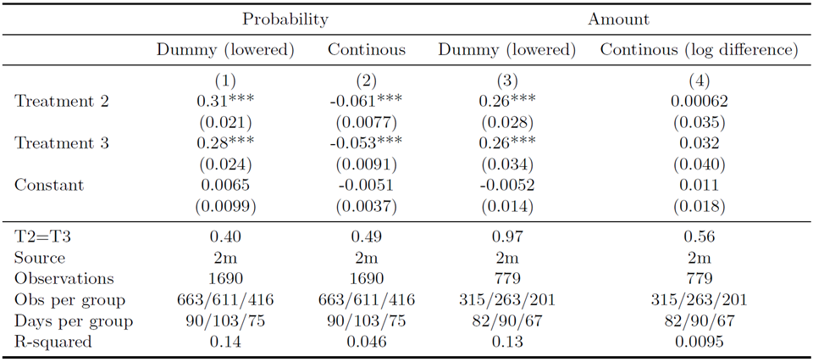
\includegraphics[width=.8\textwidth]{Tables/Table6.png}
%  \caption*{Notes: The table estimates the effect of the information treatment on immediate expectation updating. All control group observations are coded as being unchanged from baseline to follow-up, and hence the coefficients for the two treatment groups reflect a simple difference between baseline and immediate follow-up. The dependent variable in Column (1) regresses an indicator variable equal to 1 if the respondent reported a lower probability of winning from the first to the second survey, and Column (2) is the continuous variable for the change in the probability of winning across the two surveys. The dependent variable in Column (3) is an indicator that the amount the worker expected to win was lower in the second survey compared with the first, and in Column (4) is the change in the log of the amount the worker expected to win.}
%  \label{tab:6}
% \end{figure}%-----------------------------------------------

%--------------------------------------------
\begin{table}[H]
    \caption{Expectations updating} 
    \label{tab:6_TE_updating}
    \begin{center}
    \scriptsize{% Table generated by Excel2LaTeX from sheet 'te_updating'
\begin{tabular}{lcccc}
\toprule
      & \multicolumn{2}{c}{Probability} & \multicolumn{2}{c}{Amount} \\
\midrule
\midrule
      & Dummy (lowered) & Continuous (percentage) & Dummy (lowered) & Continuous (percentage) \\
\midrule
      & (1)   & (2)   & (3)   & (4) \\
\midrule
\midrule
Calculator & 0.31*** & -0.025 & 0.26*** & 2.49 \\
      & (0.020) & (0.019) & (0.029) & (2.45) \\
Calculator + letter & 0.28*** & -0.051*** & 0.25*** & 0.25* \\
      & (0.024) & (0.011) & (0.033) & (0.13) \\
Constant & 0.0077 & -0.0098 & -0.0041 & -0.69 \\
      & (0.0098) & (0.011) & (0.014) & (0.69) \\
      &       &       &       &  \\
\midrule
Observations & 1722  & 1722  & 790   & 790 \\
R-squared & 0.143 & 0.005 & 0.128 & 0.004 \\
Source & 2m    & 2m    & 2m    & 2m \\
BVC   & YES   & YES   & YES   & YES \\
Obs per group & 675/625/422 & 675/625/422 & 320/266/204 & 320/266/204 \\
Days per group & 90/103/75 & 90/103/75 & 82/91/67 & 82/91/67 \\
T2 = T3 & 0.40  & 0.25  & 0.88  & 0.36 \\
\bottomrule
\bottomrule
\end{tabular}%
}
    \end{center}
     \scriptsize {\noindent The table estimates the effect of the information treatment on immediate expectation updating. All control group observations are coded as being unchanged from baseline to follow-up, and hence the coefficients for the two treatment groups reflect a simple difference between baseline and immediate follow-up. The dependent variable in Column (1) regresses an indicator variable equal to 1 if the respondent reported a lower probability of winning from the first to the second survey, and Column (2) is the continuous variable for the change in the probability of winning across the two surveys. The dependent variable in Column (3) is an indicator that the amount the worker expected to win was lower in the second survey compared with the first, and in Column (4) is the change in the log of the amount the worker expected to win.
    \textit{Do file: } \texttt{te\_updating.do}
}
\end{table}
  
    
%--------------------------------------------


\noindent\emph{Settlement and contact with lawyers}\\
Changing expectations is an important intermediate outcome, but we are most interested in understanding whether the treatments changed the likelihood of suing and the quality of the lawyer hired in the event of suing. We use data from follow-up surveys 2 weeks and 2 months after the treatment day to measure whether the worker reports having solved the conflict or sued, and whether she had talked with any type of lawyer. Table 7 shows ITT estimates, showing that both treatments had an effect on the subsequent actions of the participants. Recall that the law specifies that workers have 60 days after dismissal to file suit, so the results using data from the two months survey (columns 2 and 4 on solving the conflict and suing, respectively) should fully capture the effect of the treatment on the decision to file a suit.

We see that the stronger treatment – the information combined with the appointment with the court’s conciliator – has a rapid and large effect on solving the conflict. After two weeks (column 1), recipients receiving the calculator and letter are 8 percentage points more likely to report that the conflict was solved, reflecting an almost 25 percent increase from the 32 percent of the control group solving their conflict over this period. By two months (column 2), the treatment effect doubles to 16 percentage points, an increase of on-third from the 50 percent rate in the control group. Information alone has no effect at two weeks, but it increases resolution by 5 percentage points (10 percent of the control group mean) after two months. These results are mirrored in the likelihood of filing a suit (column 4), suggesting that the treatment effect is coming largely from circumstances where the worker would have filed a suit (rather than drop the case) in the absence of treatment. Column 3 examines whether the worker talked to any lawyer at two weeks. While the calculator treatment had no effect, the appointment letter caused a 20 percentage point decrease in the likelihood of talking to any lawyer. The appointment letter allowed workers to bargain directly with their employer through the conciliator, giving them a concrete strategy to implement, and so obviating the need to talk with a lawyer.

The results on Table 7 indicate that the treatment had an effect on the decision to sue. We can also ask which types of cases were not filed as a result of treatment. Figure 4 shows the kernel density of value of cases, as predicted by the calculator. The left-hand figure shows the full sample for each of the three treatment groups, and the right-hand figure the distribution conditional on filing a suit. We see that the treated participants deciding not to sue come disproportionately from those with lower value cases. The fact that those with the lowest case values are most likely to decide not to sue is consistent with them realizing that they were unlikely to recover the cost of filing a suit and the opportunity cost of their time. 

%--------------------------------------------
\begin{table}[!ht]
    \caption{Effects on settlement, talking to lawyers, and suing} 
    \label{tab:7_TE_action}
    \begin{center}
    \footnotesize{% Table generated by Excel2LaTeX from sheet 'te_main_outcomes'
\begin{tabular}{lcccc}
\toprule
      & \multicolumn{2}{c}{Solved conflict} & Talked to lawyer & Sued \\
\midrule
\midrule
      & (1)   & (2)   & (3)   & (4) \\
\midrule
\midrule
Calculator & -0.018 & 0.047* & -0.0070 & -0.052* \\
      & (0.029) & (0.028) & (0.028) & (0.027) \\
Calculator + letter & 0.083** & 0.16*** & -0.20*** & -0.12*** \\
      & (0.035) & (0.032) & (0.032) & (0.031) \\
Constant & 0.34*** & 0.50*** & 0.60*** & 0.37*** \\
      & (0.025) & (0.025) & (0.026) & (0.025) \\
      &       &       &       &  \\
\midrule
Observations & 1813  & 2091  & 1814  & 2034 \\
R-squared & 0.007 & 0.022 & 0.028 & 0.014 \\
Source & 2w    & 2m    & 2w    & 2m \\
BVC   & YES   & YES   & YES   & YES \\
Obs per group & 722/668/423 & 801/759/531 & 722/669/423 & 781/741/512 \\
Days per group & 81/91/61 & 93/106/75 & 81/91/61 & 93/106/75 \\
T2 = T3 & 0.0040 & 0.00041 & 2.4e-09 & 0.016 \\
\bottomrule
\bottomrule
\end{tabular}%
}
    \end{center}
    \scriptsize {\noindent Data form the follow-up surveys at 2 weeks or 2 months, as indicated. The dependent variables correspond to survey responses to the following questions: (Solved Conflict) “Have you arrived to an agreement with your former employer?", (Talked to Lawyer) “Have you spoken to any public lawyer or any person from the public prosecutor's office or Have you spoken to any private lawyer?”, (Sued) “Did you sue your former employer?”.
    \textit{Do file: } \texttt{te\_main\_outcomes.do}}
\end{table}

%--------------------------------------------



\begin{figure}[H]%-------------------------------------------
  \centering
  \caption{Distribution of the predicted value of cases by treatment, conditional and unconditional on suing}
  \begin{minipage}[b]{0.4\textwidth}
    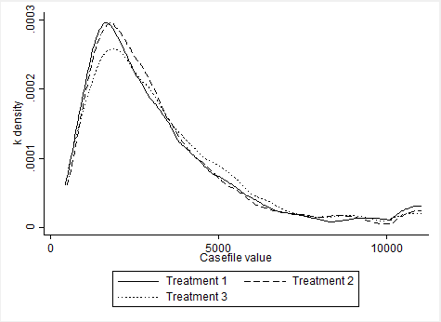
\includegraphics[width=\textwidth]{Figures/Figure4_1.png}
    \caption*{(a) Unconditional}
  \end{minipage}
  %\hfill
  \begin{minipage}[b]{0.4\textwidth}
    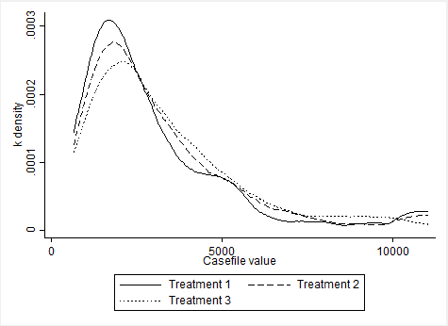
\includegraphics[width=\textwidth]{Figures/Figure4_2.png}
    \caption*{(b) Conditional on suing}
  \end{minipage}
  \label{fig:4}
\end{figure}%-------------------------------------------------

Response rates in the 2w and 2m follow up surveys are 85\% and 80\% respectively. Although we control for the basic variables of the case in all regression, we may have a selection problem on unobservables. In the appendix, we show results from Lee bounds to address this. The Lee bounds show that results for “solved conflict’’ and “sued’’ remain significant for both treatments at 2 months, as does the effect of the letter of appointment on “talked to lawyer’’.

The results on Table 7 come from the survey data. We can also estimate the effect on filing a suit using administrative data. This has the advantage of not being subject to issues with attrition. However, the administrative data introduces measurement error because the match rates are not perfect. There is noise in the matching process coming from the fact that the names of the worker or the firm may be misspelled in the case filing, or could be coded with a mistake in the court’s administrative database from which we identify the case filings. Nevertheless, our match rates are reasonably high. Among the sample workers who report having filed a suit at two months, we find almost two-thirds (63 percent) in the court records. Table 8 reports results on the suing using data from the administrative records. The first column repeats the results of column 4 from Table 7, to make the comparison easier. Column 2 shows results using a precise match on names of the worker and firm, and column 3 the results using a fuzzy match that allows for misspellings of names. Notice first that, in the control group, the proportion of workers filing a suit drops from 38 percent in the survey data to 28 percent and 30 percent in the precise and fuzzy match samples, respectively. This reflects the incomplete matching in the administrative records. Consistent with some attenuation from measurement error, the magnitude of the effect on the calculator + letter treatment is smaller, though the effect remains significant. On the other hand, the effect of the calculator on filing a suit becomes insignificant when we use the administrative data. 

%--------------------------------------------
\begin{table}[!ht]
    \caption{Effects on suing with administrative data} 
    \label{tab:8}
    \center
    \notesize{% Table generated by Excel2LaTeX from sheet 'Table 8 - sued_admin'
\centering
  %\caption{Add caption}
    \begin{tabular}{lccc}
          &       &       &  \\
    \midrule
    \midrule
          & Sued  & Sued (admin data) & Sued (admin data) \\
    \midrule
          & (1)   & (2)   & (3) \\
    \midrule
    Calculator & -0.060** & 0.014 & 0.0087 \\
          & (0.027) & (0.023) & (0.022) \\
    Calculator + letter & -0.12*** & -0.042* & -0.057** \\
          & (0.031) & (0.024) & (0.025) \\
    Constant & 0.38*** & 0.28*** & 0.30*** \\
          & (0.025) & (0.019) & (0.019) \\
    T2=T3 p-value & 0.030 & 0.017 & 0.0060 \\
    Source & 2m    & Admin exact & Admin fuzzy \\
    Observations & 1992  & 2525  & 2525 \\
    Obs per group & 765/725/502 & 991/912/622 & 991/912/622 \\
    Days per group & 93/106/75 & 94/107/77 & 94/107/77 \\
    R-squared & 0.014 & 0.0024 & 0.0035 \\
    Control gorup mean & 0.4   & 0.28  & 0.30 \\
    \bottomrule
    \bottomrule
    \end{tabular}%
 }
    \begin{figurenotes}
    This table presents the estimated treatment effects over suing for both treatment arms. Column (1) presents the effect over survey data, while columns (2) and (3) derive the outcome of suing from administrative data provided by the MCLC. All regressions control for 3 basic variables: tenure, daily wage, and gender. 
    \end{figurenotes}
    %\textit{Do file: } \texttt{}
  
\end{table}
%--------------------------------------------


\noindent\emph{Effects on Lawyer selection}\\
Besides changing the margin of suing vs. settlement, we can also study what type of lawyers workers talked to and sued with. Table 9 classifies lawyers in three types: public lawyer, informal lawyer (“coyote’’), or private formal, and explores whether our treatments had effects on which lawyers they used. We use data from the survey, and identify informal lawyers as those who the worker reports finding outside the court building. 

We hypothesize that provision of the information about what outcomes are expected leaves workers more informed and better able to select a higher-quality lawyer. The information reduces the informational asymmetries between workers and their potential lawyers, and therefore make workers more knowledgeable and potentially more ‘sophisticated’ in choosing their lawyer. They are then likely to be better equipped to tell when a lawyer is exaggerating the likelihood of winning case, and the amount they will win. As we noted above, some private lawyers seem to be inducing workers to sue by building up their expectations of probabilities and amounts of winning. Sadka et al. (2019) found that, accounting for filing fees, 40 percent of plaintiffs actually lost money on their case. Having the letter of appointment also helps them pressure employers to settle – and thus need lawyers less – and it also ensures they better understand the process of suing. 

We measure two kinds of interactions of workers with lawyers. At two weeks, we ask which types of lawyers the workers have talked with. At two months, we measure which type of lawyer they sued with, conditional on them filing a suit. For each of these we asked how exactly they found their lawyer. The responses included “at the stairs or entrance of the court’’, “through family or friends’’, “through media advertisements’’, among others.

Table 9 reports ITT results for talking to (columns 1-3) or suing with (columns 4-6) public, private informal, and private formal lawyers. These regressions estimate the causal effect of our treatment on type of lawyer, as the estimates are not conditional on any outcome (i.e., in the regressions for suing, the dependent variable is zero if they did not sue). Column 1 shows that receiving the calculator treatment reduces the likelihood of talking to a public lawyer by 12 percentage points (against the control group mean of 38 percent), but does not change the likelihood of talking to an informal lawyer. The calculator treatment increased by 8.6 percentage points the likelihood of talking to a private formal lawyer\footnote{The effects do not sum to 1 because we are not conditioning on suing.}.  Even though the information did not change the likelihood of talking to an informal lawyer, the likelihood of suing with an informal lawyer decreased by 3.3 percentage points (47 percent of the control mean). The calculator also reduced the probability of suing with a public lawyer by 5.9 percentage points, and increased the likelihood of suing with a formal private lawyer by 3.7 percentage points (28 percent of the mean). Combining the results from columns 4 through 6 shows that the calculator information caused a change in the composition of lawsuits, reducing the importance of informal private lawyers and increasing the use of formal private lawyers. 

The calculator + appointment letter treatment had even larger effects on talking to lawyers and suing, decreasing the likelihood of talking to a public lawyer by 26 percentage points and the likelihood of talking with an informal lawyer by 4 percentage points. The appointment letter appears to substitute for talking with these types of lawyers. There was no change in talking to a formal private lawyer. The effect on suing is also large: as with the calculator, the appointment letter reduced by 6 percentage points the likelihood of suing with a public lawyer, and suing with an informal lawyer by close to 4 percentage points (58 percent of the mean)\footnote{We also find strong effects conditional on talking to a lawyer. Receiving the calculator treatment reduces the likelihood of talking to a public lawyer, but it does not increase the likelihood of talking to an informal lawyer, which means that it pushes workers towards formal private representation. The effects are large 19 percentage points lower contact with public lawyers in the calculator treatment, and 33 percentage points for the letter of appointment treatment. Once workers have a letter of appointment, they may see less value on talking to a public lawyer. The effect on suing is also large: both the calculator and the appointment letter treatments reduced by 7 percentage points the likelihood of suing with an informal lawyer (35 percent of the control mean). The calculator treatment also decreased suing with public lawyer by 8pp, but the estimate is noisier.}.  There is no statistically significant evidence of a decrease in suing with a private formal lawyer. The calculator + letter treatment thus produced a similar shift in the composition of lawyers filing cases, away from informal lawyers and public lawyers and toward formal private lawyers.

%--------------------------------------------
\begin{table}[!ht]
    \caption{Effects on suing with administrative data} 
    \label{tab:9_lawyer_uncond}
    \center
    \scriptsize{% Table generated by Excel2LaTeX from sheet 'TE_lawyer_uncond_v123'
\begin{tabular}{lcccccc}
\toprule
      & \multicolumn{3}{c}{Talked} & \multicolumn{3}{c}{Sued } \\
\midrule
      & Public lawyer & Informal lawyer & Private Formal Lawyer & Public lawyer & Informal lawyer & \multicolumn{1}{l}{Private Formal Lawyer} \\
\midrule
      & (1)   & (2)   & (3)   & (4)   & (5)   & (6) \\
Treatment 2 & -0.12*** & 0.0050 & 0.086*** & -0.059*** & -0.033*** & 0.037** \\
      & (0.029) & (0.013) & (0.026) & (0.020) & (0.011) & (0.017) \\
Treatment 3 & -0.26*** & -0.039*** & 0.021 & -0.056** & -0.041*** & -0.026 \\
      & (0.029) & (0.013) & (0.029) & (0.022) & (0.012) & (0.018) \\
Constant & 0.40*** & 0.073*** & 0.24*** & 0.19*** & 0.074*** & 0.10*** \\
      & (0.024) & (0.013) & (0.026) & (0.018) & (0.011) & (0.014) \\
T2=T3 & 0.00000043 & 0.00051 & 0.021 & 0.91  & 0.43  & 0.0010 \\
\midrule
Source & 2w    & 2w    & 2w    & 2m    & 2m    & 2m \\
Observations & 1814  & 1814  & 1814  & 2057  & 2057  & 2057 \\
Obs per group & 722/669/423 & 722/669/423 & 722/669/423 & 788/744/525 & 788/744/525 & 788/744/525 \\
Days per group & 81/91/61 & 81/91/61 & 81/91/61 & 93/106/75 & 93/106/75 & 93/106/75 \\
R-squared & 0.055 & 0.010 & 0.013 & 0.011 & 0.011 & 0.0089 \\
Control group mean & 0.38  & 0.07  & 0.28  & 0.2   & 0.07  & 0.12 \\
\bottomrule
\bottomrule
\end{tabular}%
}
    \begin{figurenotes}
    Columns 1 through 3 use responses from the two-week survey asking if the worker had talked with a lawyer and, if so, where they found the lawyer. Columns 4-6 use data from the two-month survey asking if the worker had sued, and if so, where they found their lawyer. The regressions are intention-to-treat, based on assignment to treatment.
    \end{figurenotes}
    %\textit{Do file: } \texttt{lawyer_uncond}
  
\end{table}


\begin{table}[!ht]
    \caption{Effects on suing} 
    \label{tab:9_lawyer_uncond}
    \center
    \scriptsize{% Table generated by Excel2LaTeX from sheet 'effects_on_suing'
\begin{tabular}{lccccccc}
\toprule
      & \multicolumn{3}{c}{Talked} &       & \multicolumn{3}{c}{Sued} \\
\midrule
\midrule
      & Public lawyer & Private formal & Private informal &       & Public lawyer & Private formal & Private informal \\
\cmidrule{2-4}\cmidrule{6-8}      & (1)   & (2)   & (3)   &       & (4)   & (5)   & (6) \\
\midrule
\midrule
Calculator & -0.12*** & 0.088*** & -0.088*** &       & -0.058*** & 0.042** & -0.042** \\
      & (0.029) & (0.026) & (0.026) &       & (0.021) & (0.018) & (0.018) \\
Calculator + letter & -0.27*** & 0.021 & -0.021 &       & -0.057** & -0.025 & 0.025 \\
      & (0.029) & (0.030) & (0.030) &       & (0.023) & (0.018) & (0.018) \\
      &       &       &       &       &       &       &  \\
\midrule
Observations & 1779  & 1777  & 1777  &       & 2019  & 2032  & 2032 \\
R-squared & 0.056 & 0.015 & 0.015 &       & 0.012 & 0.009 & 0.009 \\
Source & 2w    & 2w    & 2w    &       & 2m    & 2m    & 2m \\
BVC   & YES   & YES   & YES   &       & YES   & YES   & YES \\
Obs per group & 709/655/415 & 708/655/414 & 708/655/414 &       & 776/735/508 & 779/742/511 & 779/742/511 \\
Days per group & 80/91/61 & 80/91/61 & 80/91/61 &       & 93/106/75 & 93/106/75 & 93/106/75 \\
Control Mean & 0.38  & 0.28  & 0.72  &       & 0.2   & 0.12  & 0.88 \\
T2 = T3 & 0     & 0.02  & 0.02  &       & 0.94  & 0     & 0 \\
\bottomrule
\bottomrule
\end{tabular}%
}
    \begin{figurenotes}
    Columns 1 through 3 use responses from the two-week survey asking if the worker had talked with a lawyer and, if so, where they found the lawyer. Columns 4-6 use data from the two-month survey asking if the worker had sued, and if so, where they found their lawyer. The regressions are intention-to-treat, based on assignment to treatment.
    \end{figurenotes}
    %\textit{Do file: } \texttt{lawyer_uncond}
  
\end{table}
%--------------------------------------------

Table 3 and 4 showed that, measured either by outcomes or inputs, informal lawyers are of lower quality than either formal private or public lawyers. On average, public and formal private lawyers appear to be of similar quality, though public lawyer appear to settle more cases. The shifts away from informal lawyers clearly suggests a movement in the direction of higher-quality representation for clients. The shift away from public lawyers is ambiguous with respect to lawyer quality, though we might expect this to result in the settling of fewer suits\footnote{ On the other hand, the reduction in the number of suits filed reduces the burden on the court, and hence the net effect on the treatment appears to be positive in this regard as well. }.  

Both treatments increased the share of lawsuits that were filed by formal private lawyers. This aggregate causal effect might be driven by either a change in the composition of workers that sue (selection induced by the treatment), or by the treatment effect on a given worker. Both effects may weigh in the coefficient estimate. For instance, those that have lower-value cases may decide not to sue after they learn this value, since they incur fixed costs from suing (fees or the time and disutility of going to court). In this case we may be changing the composition of what cases go to court. On the other hand, if the treated learn that their case is valuable enough, they may decide to sue with a higher-quality (perhaps higher-priced) lawyer. Note that we control for the plaintiff’s daily wage, tenure in the firm, worker age, and gender. So if selection occurs only in on these margins, the results in Table 9 would be close to the treatment effect on a given worker. In a future version of the paper, we will attempt to identify a subsample of “always suers”, and test whether within this subsample, those in the treatment group sue with different types of lawyers. We plan to begin by examining heterogeneous treatment effects on suing, using the method proposed by Athey and Imbens (2015). This may give us insight into sub-samples where the treatment lead to no selection effects on suing. 

For now, we use the predicted case ratings to estimate the effect of the treatments on the quality of the case file, ignoring the selection effects. This is intended only to detail the proposed method. As we have not addressed the selection issues, we should not put much weight on the specific results we present on this. 
\\

\noindent\emph{Effects on Quality of the Case File}\\
The fact that the share of lawsuits filed by informal lawyers decreases with treatment is a strong indication that the treatments improve the quality of lawsuits that reach the court. Moreover, we believe that the reduction in the percentage of cases filed by informal lawyers represents an improvement in the functioning of the institution, particularly given the evidence of nefarious actions by informal lawyers. However, we would like to understand the effect of the treatments on the quality of case filings more generally. The direct way to do this is to have each of the filed cases rated by practicing lawyers, as we did for the 500 historical case files. Because the experiment ended relatively recently, we have not yet completed this exercise. Instead, for now we estimate the effect of treatments on the predicted quality of the cases filed by plaintiffs participating in the experiment. We predict the values in the same manner as we described above, using the 40 coded variables mapped to the subjective ratings of the 500 historical case filings. 

This exercise has limitations that should be kept in mind. First, the prediction introduces error in the dependent variable of the regression. More importantly, there are selection effects that, for now, we ignore. We only observe cases - and therefore case file quality – conditional on suing. Table 7 showed effects on the extensive margin, especially for the calculator + conciliator letter treatment. As a consequence, these results may be subject to a selection issues, as different kinds of workers may be suing on the different treatment arms, and at the same time different types of workers may choose different kinds of lawyers.
\\
%--------------------------------------------
\begin{table}[!ht]
    \caption{Predicted quality of case file conditional on suing} 
    \label{tab:10_TE_quality_postlasso}
    \center
    \scriptsize{% Table generated by Excel2LaTeX from sheet 'T10-TE_quality'

  \centering
  %\caption{Add caption}
    \begin{tabular}{lrrr}
    \midrule
    \midrule
          & \multicolumn{1}{c}{(2)} & \multicolumn{1}{c}{(4)} & \multicolumn{1}{c}{(6)} \\
          &       &       & \multicolumn{1}{c}{\multirow{2}[1]{*}{Reported suing, private lawyer}} \\
    Variables & \multicolumn{1}{c}{Whole sample} & \multicolumn{1}{c}{Reported Suing} &  \\
    \midrule
          &       &       &  \\
    Calculator (T2) & \multicolumn{1}{c}{-0.0181} & \multicolumn{1}{c}{-0.0353} & \multicolumn{1}{c}{-0.00314} \\
          & \multicolumn{1}{c}{(0.044)} & \multicolumn{1}{c}{(0.057)} & \multicolumn{1}{c}{(0.085)} \\
    Calculator + Letter (T3) & \multicolumn{1}{c}{0.00449} & \multicolumn{1}{c}{0.104} & \multicolumn{1}{c}{0.236} \\
          & \multicolumn{1}{c}{(0.128)} & \multicolumn{1}{c}{(0.174)} & \multicolumn{1}{c}{(0.342)} \\
    Constant & \multicolumn{1}{c}{7.919***} & \multicolumn{1}{c}{7.926***} & \multicolumn{1}{c}{7.671***} \\
          & \multicolumn{1}{c}{(0.037)} & \multicolumn{1}{c}{(0.043)} & \multicolumn{1}{c}{(0.102)} \\
          &       &       &  \\
    \midrule
    Observations & \multicolumn{1}{c}{694} & \multicolumn{1}{c}{497} & \multicolumn{1}{c}{266} \\
    R-squared & \multicolumn{1}{c}{0.004} & \multicolumn{1}{c}{0.007} & \multicolumn{1}{c}{0.018} \\
    BVC   & \multicolumn{1}{c}{Yes} & \multicolumn{1}{c}{Yes} & \multicolumn{1}{c}{Yes} \\
    Source & \multicolumn{1}{c}{2m} & \multicolumn{1}{c}{2m} & \multicolumn{1}{c}{2m} \\
    Obs. per group & \multicolumn{1}{c}{288/265/141} & \multicolumn{1}{c}{209/187/101} & \multicolumn{1}{c}{108/106/52} \\
    Days per group & \multicolumn{1}{c}{79/87/59} & \multicolumn{1}{c}{67/77/48} & \multicolumn{1}{c}{52/56/33} \\
    F-stat T2=T3 & \multicolumn{1}{c}{0.0336} & \multicolumn{1}{c}{0.695} & \multicolumn{1}{c}{0.559} \\
    p-value & \multicolumn{1}{c}{0.855} & \multicolumn{1}{c}{0.406} & \multicolumn{1}{c}{0.456} \\
    Dep. var mean & \multicolumn{1}{c}{7.924} & \multicolumn{1}{c}{7.964} & \multicolumn{1}{c}{7.836} \\
    \midrule
    \midrule
    Robust standard errors in parentheses &       &       &  \\
    *** p$<$0.01, ** p$<$0.05, * p$<$0.1 &       &       &  \\
    \end{tabular}%

}
    %\textit{Do file: } \texttt{ql\}
  
\end{table}
%--------------------------------------------


With these limitations in mind, Table 10 shows that the predicted quality of the case file is not significantly related to either treatment. The coefficients are all close to zero, indicating slightly worse predicted case quality for the calculator only treatment and slightly better case file quality for the calculator + letter treatment.
\\

\noindent\emph{Effects on welfare proxies}
Tables 7, 8 and 9 show that workers in the treatment groups are more likely to resolve their conflicts than those in the control group. This effect is particularly strong for those receiving both the calculator and letter. Ultimately, we would like to know whether the worker’s welfare was increased as a result of the treatments. We measure short-term welfare effects using several proxies obtained from the two-month survey. Our first proxy is the World Value Survey measure of happiness: “On a scale of 1 to 10, in which 1 means “not happy at all" and 10 means “totally happy", in general, how happy do you feel about your life lately?” We also asked two more objective proxies of financial hardship: “In the past three months have you had to stop paying for a basic services such as electric power, water, or rent due to lack of money?’’, and: “In the past 3 months, have you lacked money to spend on food one or more days?’’ 

In Table 11, we show the results of regressing the answers to these three questions against assignment to one of the two treatment arms or to control. At least in the short run, the treatments appear to have significantly reduced financial hardship. We find that both treatments decreased financial hardship measured by either of the two financial hardship questions by around 7 percentage points (close to 12 percent of the mean). We do not know the exact mechanism through which financial hardship is reduced, but one possibility is that the income from settlement and the lower expenses in lawyer fees and costs of going to the court and finding lawyers liberates income to pay for services and food. The results for happiness are more nuanced. Happiness increased by 0.13 and 0.29 points in the calculator and calculator plus letter treatments, respectively, though only the second of these is statistically significant. These compare with a control group mean of 8.02 (and standard deviation of 2.12). 

Table 11 shows two other outcomes related to time use of the workers. If the treatments increase settlement, we might expect that they reduce the amount of time workers spend on their case and, by doing so, increase the amount of time available for job search. We examine whether the treatment increased the likelihood they were working two months after the intervention. By inducing faster settlement, the treatments may make speed the return to work by freeing time for job search. On the other hand, the liquidity settlement may allow workers to search for a job for a longer time. In any event, while 56 percent of the control group were working again after two months, we do not find any significant effect of treatment on this outcome. Finally, we conjectured that treatments may decrease the time spent on activities related to their case. To measure this we asked: “Since the day you were fired until today, approximately how many hours have you spent trying to solve your conflict, make inquiries, follow the lawsuit process, or assisting to paperwork and related appointments?” We find a small increase in the amount of time they spent at the court. Compared with the control group mean of 17.3 hours, the treatments have modest effects, with the calculator treatment showing an increase of 1.1 hours, significant at the 10 percent level. We posit that this reflects a short-run effect, as the conciliation meeting and time to register settlements may be increasing the time spent at the court in the short run.

% \begin{figure}[hp]%-----------------------------------------
%  \centering
%  \captionof{table}{Welfare effects at 2 months}
%  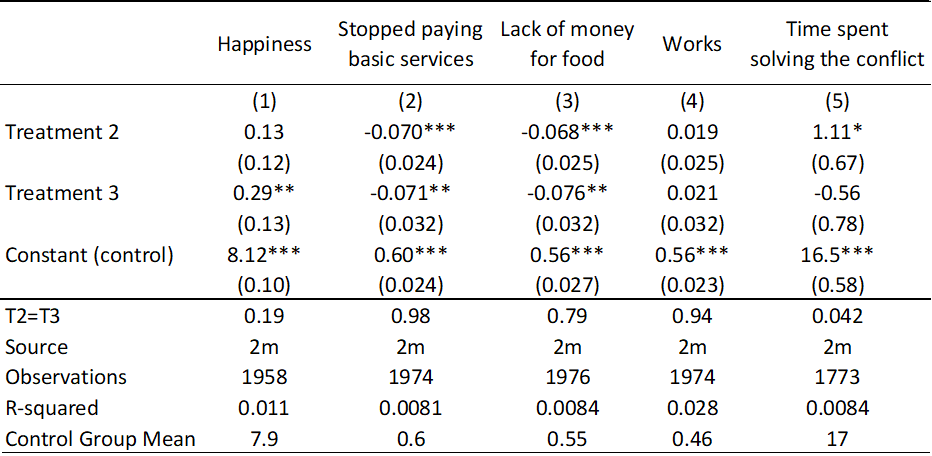
\includegraphics[width=.8\textwidth]{Tables/Table11.png}
%  \caption*{Notes: In the 2 month survey we included a battery of questions in an attempt to measure welfare proxies. In particular, we asked (Happiness) “On a scale of 1 t 10, in which 1 means “not happy at all" and 10 means “totally happy", in general, how happy do you feel about your life lately?” (Stopped paying serv.) “In the past three months have you had to stop paying for a basic service such as electric power, water, or rent due to lack of money?” (Lack of money for food) “In the past 3 months, have you lacked money to spend on food one or more days?” (Works) “Are you currently working?” (Time spent at the court) “Since the day you were fired until today, approximately how many hours have you spent trying to solve your conflict, make inquiries, follow the lawsuit process, or assisting to paperwork and related appointments?”}
%  \label{tab:11}
% \end{figure}%-----------------------------------------------

%--------------------------------------------
\begin{table}[!ht]
    \caption{Welfare effects at 2 months} 
    \label{tab:11_welfare}
    \center
    \scriptsize{% Table generated by Excel2LaTeX from sheet 'welfare_reg'
\begin{tabular}{lccccc}
\toprule
      & Happiness & Stopped paying serv.  & Lack of money for food & Works & \multicolumn{1}{p{7.165em}}{Time spent\newline{}solving the conflict} \\
\midrule
      & (1)   & (2)   & (3)   & (4)   & (5) \\
Treatment 2 & 0.13  & -0.070*** & -0.068*** & 0.019 & 1.11* \\
      & (0.12) & (0.024) & (0.025) & (0.025) & (0.67) \\
Treatment 3 & 0.29** & -0.072** & -0.077** & 0.020 & -0.60 \\
      & (0.13) & (0.032) & (0.032) & (0.032) & (0.78) \\
Constant (control) & 8.12*** & 0.60*** & 0.56*** & 0.56*** & 16.5*** \\
      & (0.10) & (0.024) & (0.027) & (0.023) & (0.58) \\
\midrule
T2=T3 & 0.18  & 0.95  & 0.77  & 0.96  & 0.039 \\
Source & 2m    & 2m    & 2m    & 2m    & 2m \\
Observations & 1959  & 1975  & 1977  & 1975  & 1774 \\
R-squared & 0.011 & 0.0081 & 0.0084 & 0.028 & 0.0086 \\
Control group mean & 7.9   & 0.6   & 0.55  & 0.46  & 17 \\
\bottomrule
\bottomrule
\end{tabular}%}
    \begin{figurenotes}
    In the 2 month survey we included a battery of questions in an attempt to measure welfare proxies. In particular, we asked (Happiness) “On a scale of 1 t 10, in which 1 means “not happy at all" and 10 means “totally happy", in general, how happy do you feel about your life lately?” (Stopped paying serv.) “In the past three months have you had to stop paying for a basic service such as electric power, water, or rent due to lack of money?” (Lack of money for food) “In the past 3 months, have you lacked money to spend on food one or more days?” (Works) “Are you currently working?” (Time spent at the court) “Since the day you were fired until today, approximately how many hours have you spent trying to solve your conflict, make inquiries, follow the lawsuit process, or assisting to paperwork and related appointments?”
    \end{figurenotes}
    %\textit{Do file: } \texttt{welfare}
  
\end{table}
%--------------------------------------------

\section{Conclusions}
Our experiment was motivated by the findings from earlier experiments in the same court (Sadka et al., 2019) that showed that private lawyers do not transmit information to their clients, and that their clients lose money in more than 40 percent of the cases. In those experiments, we intervened in ongoing cases, after plaintiffs had contracted with their lawyers. Those findings, combined with anecdotal evidence that there is a large variation in the quality of private lawyers suggested to us that we needed to intervene before workers contracted with lawyers. Our experiment aimed to test whether giving workers information before they hire a lawyer leads them to select higher quality lawyers, perhaps by making them less vulnerable by manipulation and better able to assess lawyer quality.

We find that workers coming to the court seeking information are overconfident at least in the probability they will win their case. The predicted case outcomes we provided them leads them to lower their expectations. The calculator treatment also leads to an increase in pre-filing settlements, and so a reduction in the number of lawsuits. We find that this reduction in lawsuits comes disproportionately from lower (predicted) value cases. Using our proxies of welfare we find improvements in at least some measures of welfare.

We expected the treatment would lead to selection of higher-quality lawyers, conditional on suing. We show that informal lawyers, those who capture clients at the steps of the courthouse, are lower quality by several measures, and that, indeed, the treatments push workers away from these lower-quality lawyers. The treatments also appear to push workers away from public attorneys, and future analysis will attempt to assess whether this represents optimal behavior given changes in the expected value of the case filing, or whether this is an unintended consequence of the way that treatments are delivered. If it is the latter, then a policy implication of the work would be that the information we provided under the branding of the court itself might be instead better provided under the branding of the public attorney’s office. 

Ultimately, we are interested in whether the selection of lawyer affects the plaintiff’s outcome, including both the pre-suit settlements and the outcomes from filed cases. Although most settlements occur within the first 18 months of filing, court judgments often take three of four years. We are optimistic that we will be able to follow cases over the long run and measure the ultimate case outcomes.

An ancillary, but we think interesting, contribution of the paper is the attempt to measure quality not by the outcomes of the case but by the ratings of experts looking at the case file. This serves both to validate the objective measures of quality we pre-selected, but also to try to deal with the non-random selection of cases to lawyers, isolating the case from the case file by looking at specificity (a proxy for lawyer effort) directly.





%\singlespacing
%\setlength\bibsep{0pt}
\nocite{*}
\bibliographystyle{aea}
\bibliography{bibliography.bib}



\clearpage

\onehalfspacing

\section*{Appendix 1: Additional Figures and Tables}

%----------------------------------------------------------
\begin{figure}[!htbp] 
    \caption{Flow chart for treatment protocol}
    \centering
    %\captionsetup{singlelinecheck = false}
    %\caption*{\qquad \qquad (a)	Amount won as a	\qquad \qquad \qquad (b) Recovered a positive amount\\
    %\qquad \qquad percentage of amount asked}
    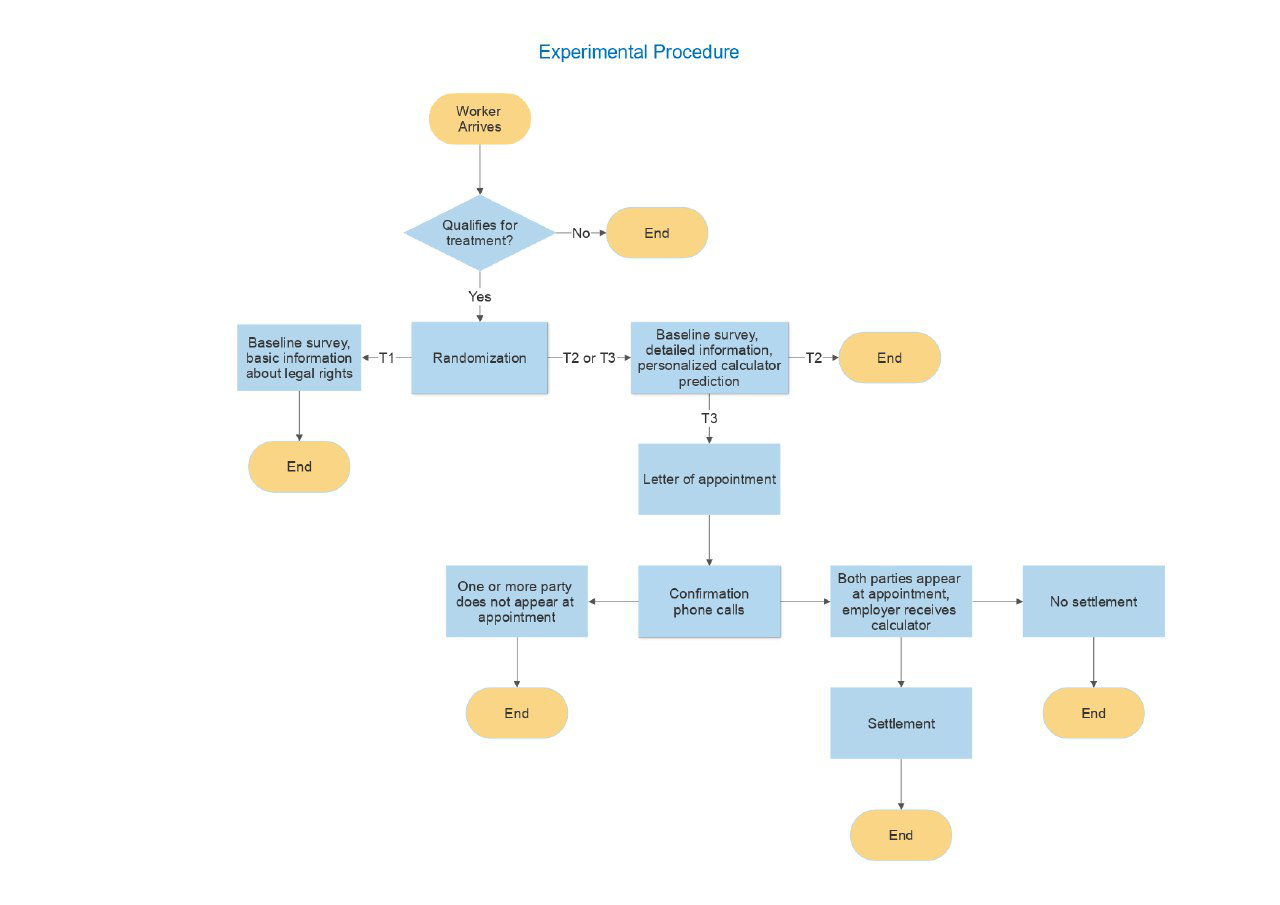
\includegraphics[width=1\textwidth]{Figures/A1_flowchart.png}
    \label{fig:A1_1}
\end{figure}
%----------------------------------------------------------
\begin{figure}[H] 
  \centering
  \caption{Lee bounds on treatment effects}
  \begin{minipage}[b]{0.4\textwidth}
    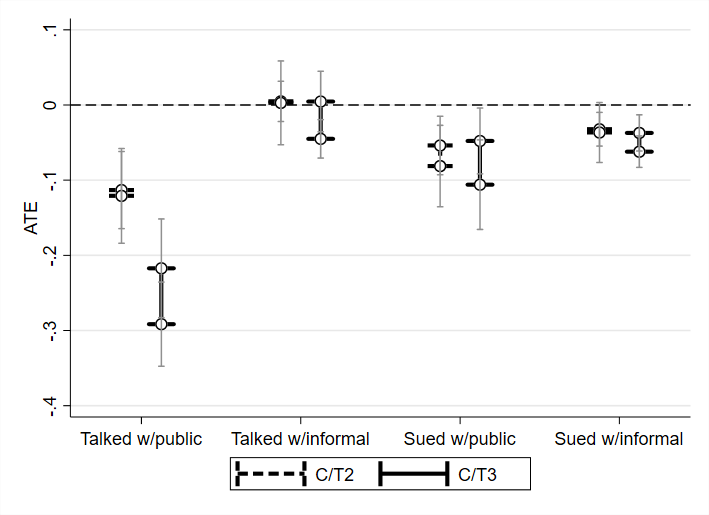
\includegraphics[width=\textwidth]{Figures/A1_fig5_1.png}
  \end{minipage}
  %\hfill
  \begin{minipage}[b]{0.4\textwidth}
    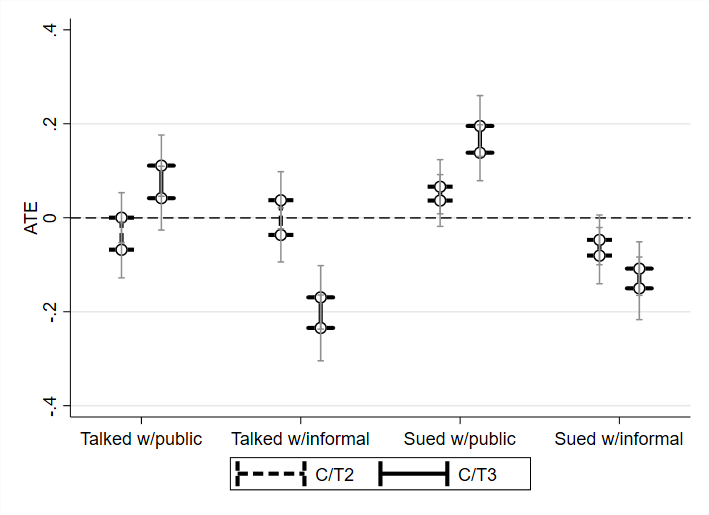
\includegraphics[width=\textwidth]{Figures/A1_fig5_2.png}
  \end{minipage}
  \label{fig:A1_fig5}
  \begin{figurenotes}
  Our survey measures of outcomes are subject to attrition. In the two weeks survey we have 367 attritors, this affects solved conflict (2w) and talked to lawyer. In the two months survey we have 540 attritors, which affects the variable sued. For the attritors in the two months survey who solved conflict after two weeks we impute the missing information from the 2w survey. This leaves 474 attritors for solved conflict(2m) in the information experiment and 400 in the lawyer inducement experiment. We implement lee bounds to take this attrition into account. This figure displays the bounds for the treatment effect (i.e. with respect to the control group T1 for the information experiment and A for the lawyer inducement experiment) along with their 95 percent confidence intervals. For each outcome we report 3 treatment effects. All significant results in Table 2 for T2 are robust to lee bounds. For T3 solved conflict at 2w and sued is not robust. For treatment B the effect on talked two lawyer is robust.
  \end{figurenotes}
\end{figure}
%----------------------------------------------------------
%Faltan tablas: attrition y find_lawyer
\section*{Appendix 2: Treatments}

i) Control Treatment
%----------------------------------------------------------
\begin{figure}[H] 
    %\caption{Control Treatment}
    \centering
    %\captionsetup{singlelinecheck = false}
    %\caption*{\qquad \qquad (a)	Amount won as a	\qquad \qquad \qquad (b) Recovered a positive amount\\
    %\qquad \qquad percentage of amount asked}
    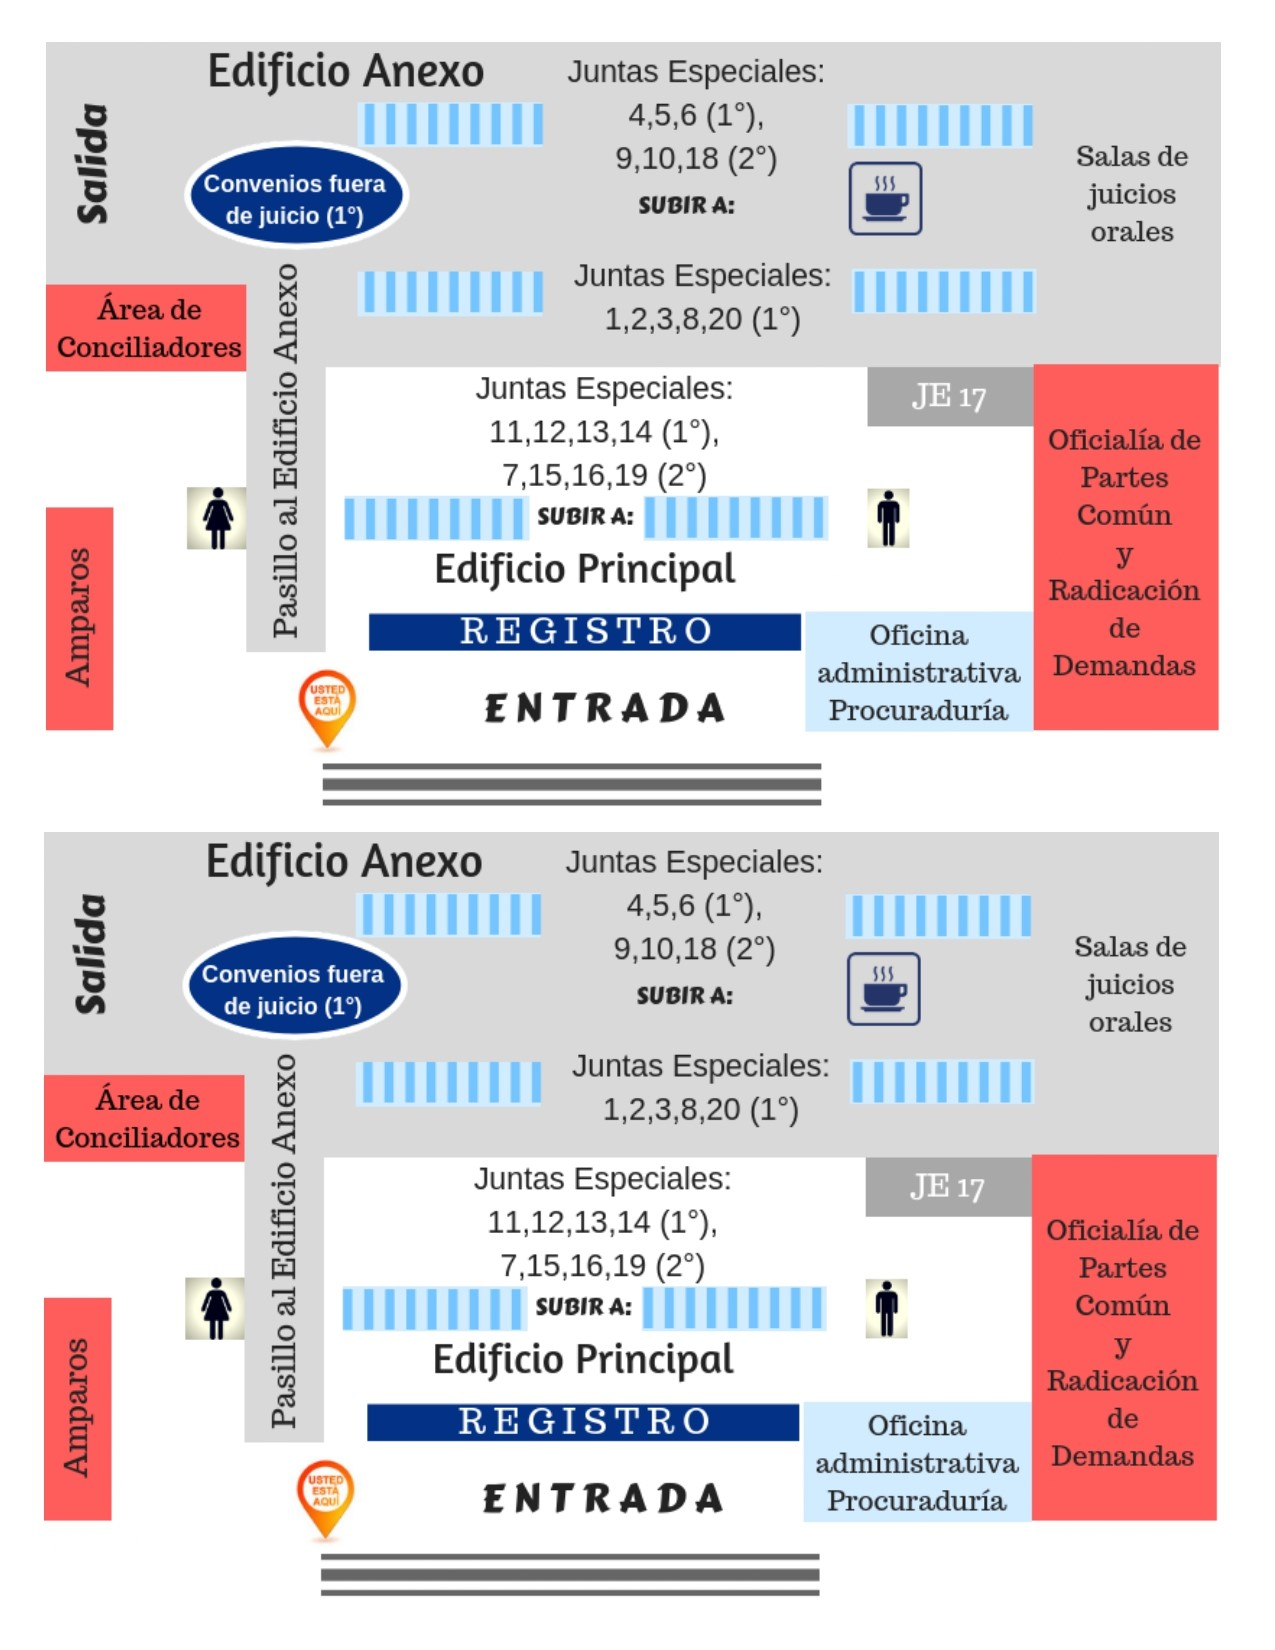
\includegraphics[width=0.8\textwidth]{Figures/A2_controlTreatment.jpg}
    \label{fig:A2_1}
\end{figure}
%----------------------------------------------------------
\begin{figure}[H] %!htbp
    %\caption{Control Treatment}
    \centering
    %\captionsetup{singlelinecheck = false}
    %\caption*{\qquad \qquad (a)	Amount won as a	\qquad \qquad \qquad (b) Recovered a positive amount\\
    %\qquad \qquad percentage of amount asked}
    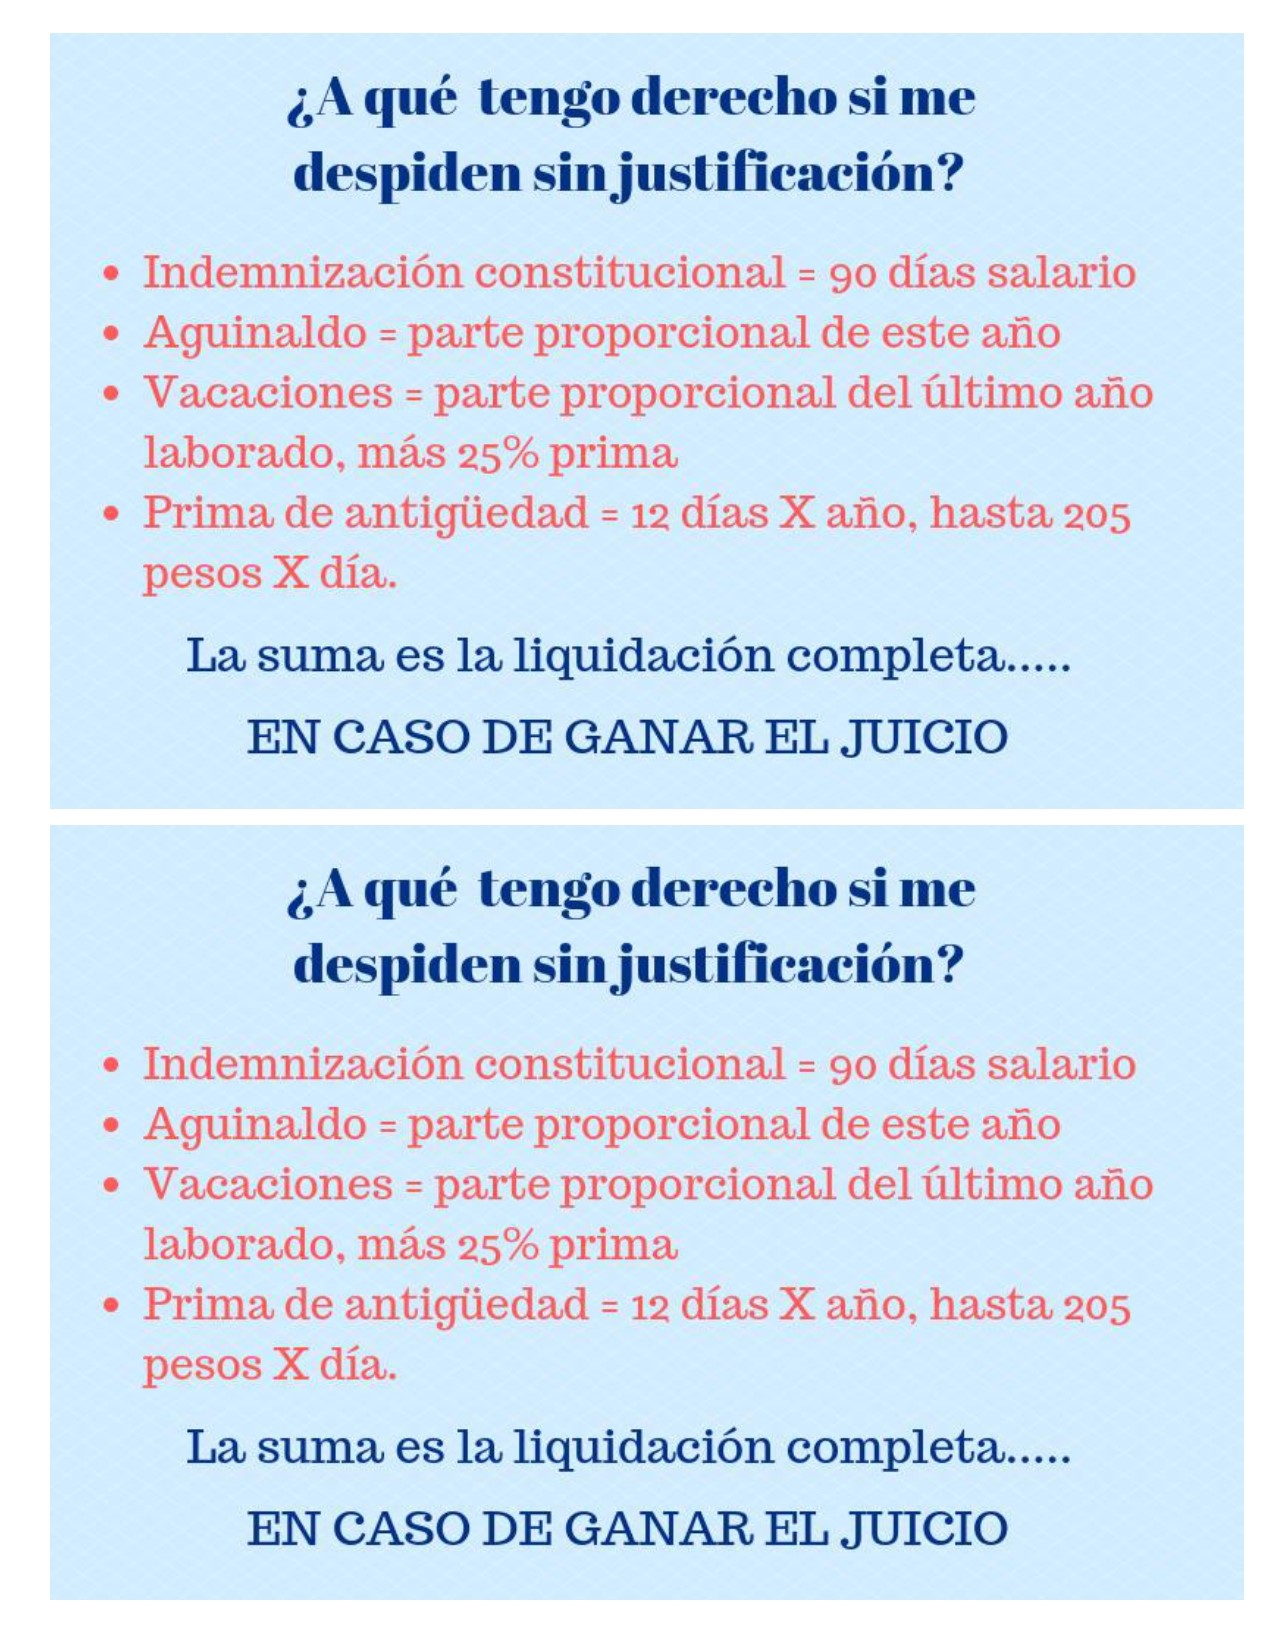
\includegraphics[width=0.8\textwidth]{Figures/A2_derechosDespido.jpg}
    \label{fig:A2_2}
\end{figure}
%----------------------------------------------------------



ii) Additional information provided in treatments 2 and 3\\
%----------------------------------------------------------
\begin{figure}[H] 
  \centering
  \begin{minipage}[b]{0.45\textwidth}
    
\includegraphics[width=\textwidth]{Figures/A2_1.jpg}
  \end{minipage}
  %\hfill
  \begin{minipage}[b]{0.45\textwidth}
    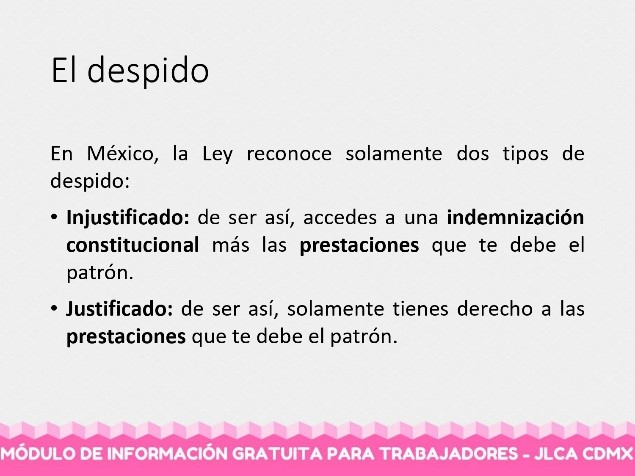
\includegraphics[width=\textwidth]{Figures/A2_2.jpg}
  \end{minipage}
  \label{fig:A2_3_1}
\end{figure}
%----------------------------------------------------------
\begin{figure}[H] 
  \centering
  \begin{minipage}[b]{0.45\textwidth}
    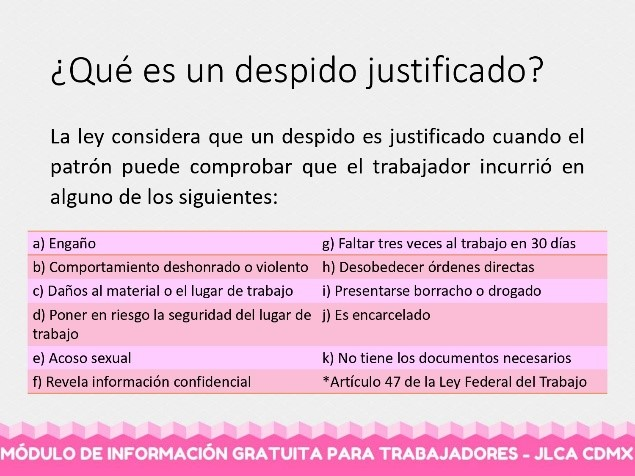
\includegraphics[width=\textwidth]{Figures/A2_3.jpg}
  \end{minipage}
  %\hfill
  \begin{minipage}[b]{0.45\textwidth}
    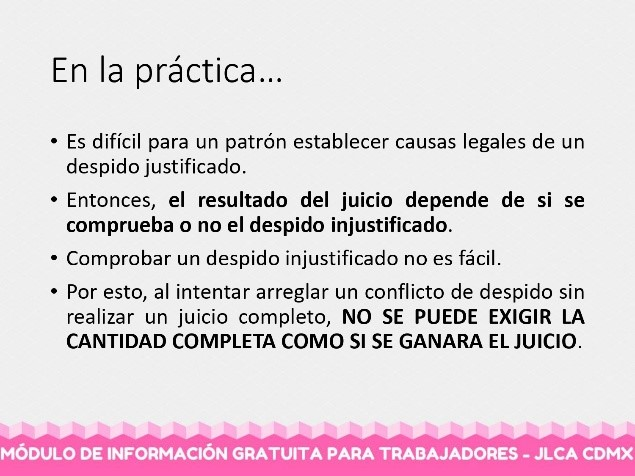
\includegraphics[width=\textwidth]{Figures/A2_4.jpg}
  \end{minipage}
  \label{fig:A2_3_2}
\end{figure}
%----------------------------------------------------------
\begin{figure}[H] 
  \centering
  \begin{minipage}[b]{0.45\textwidth}
    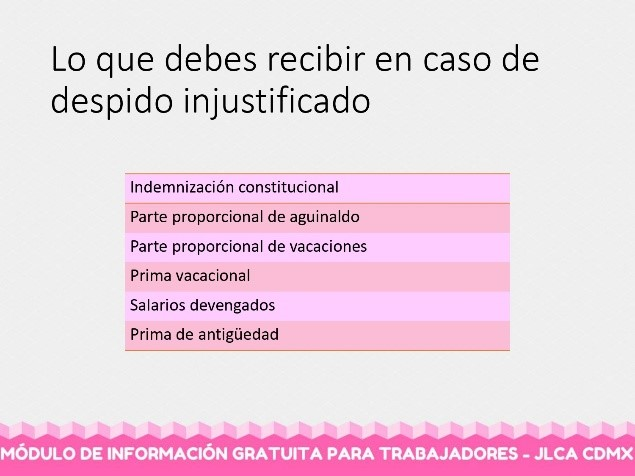
\includegraphics[width=\textwidth]{Figures/A2_5.jpg}
  \end{minipage}
  %\hfill
  \begin{minipage}[b]{0.45\textwidth}
    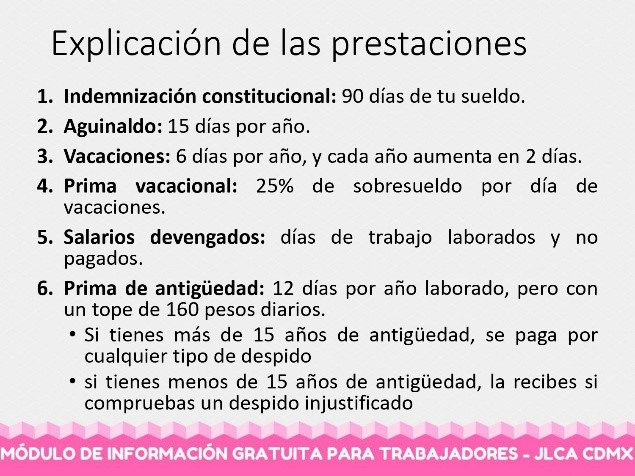
\includegraphics[width=\textwidth]{Figures/A2_6.jpg}
  \end{minipage}
  \label{fig:A2_3_3}
\end{figure}
%----------------------------------------------------------
\begin{figure}[H] 
  \centering
  \begin{minipage}[b]{0.45\textwidth}
    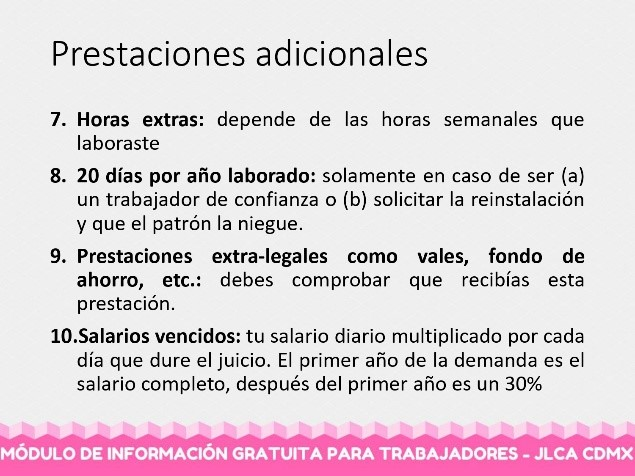
\includegraphics[width=\textwidth]{Figures/A2_7.jpg}
  \end{minipage}
  %\hfill
  \begin{minipage}[b]{0.45\textwidth}
    
\includegraphics[width=\textwidth]{Figures/A2_8.jpg}
  \end{minipage}
  \label{fig:A2_3_4}
\end{figure}
%----------------------------------------------------------
\begin{figure}[H] 
  \centering
  \begin{minipage}[b]{0.45\textwidth}
    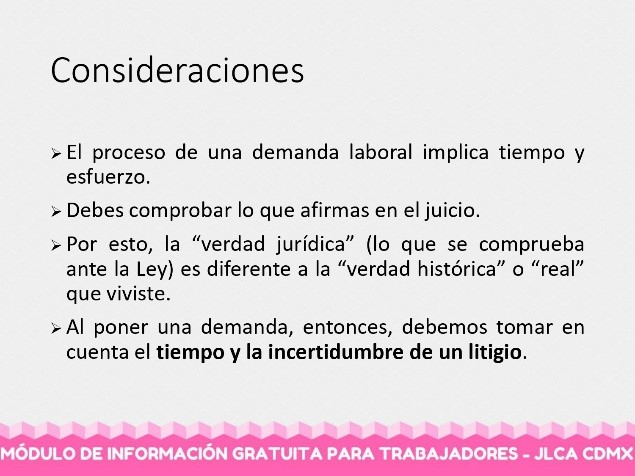
\includegraphics[width=\textwidth]{Figures/A2_9.jpg}
  \end{minipage}
  %\hfill
  \begin{minipage}[b]{0.45\textwidth}
    
\includegraphics[width=\textwidth]{Figures/A2_10.jpg}
  \end{minipage}
  \label{fig:A2_3_5}
\end{figure}
%----------------------------------------------------------
\begin{figure}[H] 
    %\caption{Control Treatment}
    \centering
    
\includegraphics[width=0.4\textwidth]{Figures/A2_11.jpg}
    \label{fig:A2_3_6}
\end{figure}
%----------------------------------------------------------
iii) Letter of appointment with the conciliator (treatment 3)
%----------------------------------------------------------
\begin{figure}[H] 
    \centering
    
\includegraphics[width=1\textwidth]{Figures/A2_letter_ES.PNG}
    \label{fig:A2_4_1}
\end{figure}
%----------------------------------------------------------
\begin{figure}[H] 
    \centering
    
\includegraphics[width=1\textwidth]{Figures/A2_letter_EN.PNG}
    \label{fig:A2_4_2}
\end{figure}
%----------------------------------------------------------


%-------------------------------------------------------------




\clearpage


% \begin{figure}[hp]%-----------------------------------------
%  \centering
%  \captionof{table}{Summary Statistics and Balance}
%  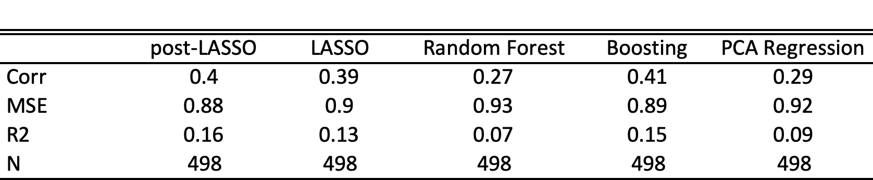
\includegraphics[width=.8\textwidth]{Table2.png}
%  \caption*{Notes: The table shows goodness-of-fit statistics: correlation of predicted vs. actual subjective quality; mean square error and out-of-sample R square in a regression of predicted vs. actual subjective quality.}
%  \label{tab:2}
% \end{figure}%-----------------------------------------------


%\begin{figure}[hp]
%  \centering
%  \includegraphics[width=.8\textwidth]{../fig/placeholder.pdf}
%  \caption{Placeholder}
%  \label{fig:placeholder}
%\end{figure}




\clearpage



\end{document}